% vim: set spell spelllang=en tw=100 et sw=4 sts=4 foldmethod=marker foldmarker={{{,}}} :

\documentclass[aspectratio=169,compress,10pt]{beamer}

\usepackage{tikz}
\usepackage{xcolor}
\usepackage{complexity}
\usepackage{hyperref}
\usepackage{microtype}
\usepackage{amsmath}                   % \operatorname
\usepackage{amsfonts}                  % \mathcal
\usepackage{amssymb}                   % \nexists
\usepackage[vlined]{algorithm2e} % algorithms
\usepackage{centernot}
\usepackage{listings}
\usepackage{csquotes}
\usepackage{fancyvrb}
\usepackage{bussproofs}
\usepackage{multicol}
\usepackage{booktabs}
\usepackage{mathtools}
\usepackage{pifont}
\usepackage{marvosym}
\usepackage{cancel}
\usepackage{nicefrac}

\usefonttheme{professionalfonts}

\usetikzlibrary{shapes, arrows, shadows, calc, positioning, fit, decorations.pathreplacing,
decorations.pathmorphing, shapes.misc, tikzmark, backgrounds, trees, overlay-beamer-styles}

\tikzset{processarrow/.style={->, very thick, decorate, decoration={snake, post length=0.5mm}}}
\tikzset{brace/.style={decorate, decoration={brace}, very thick}}

\definecolor{uofguniversityblue}{rgb}{0, 0.219608, 0.396078}
\definecolor{uofgheather}{rgb}{0.356863, 0.32549, 0.490196}
\definecolor{uofgaquamarine}{rgb}{0.603922, 0.72549, 0.678431}
\definecolor{uofgslate}{rgb}{0.309804, 0.34902, 0.380392}
\definecolor{uofgrose}{rgb}{0.823529, 0.470588, 0.709804}
\definecolor{uofgmocha}{rgb}{0.709804, 0.564706, 0.47451}
\definecolor{uofgsandstone}{rgb}{0.321569, 0.278431, 0.231373}
\definecolor{uofgforest}{rgb}{0, 0.2, 0.129412}
\definecolor{uofglawn}{rgb}{0.517647, 0.741176, 0}
\definecolor{uofgcobalt}{rgb}{0, 0.615686, 0.92549}
\definecolor{uofgturquoise}{rgb}{0, 0.709804, 0.819608}
\definecolor{uofgsunshine}{rgb}{1.0, 0.862745, 0.211765}
\definecolor{uofgpumpkin}{rgb}{1.0, 0.72549, 0.282353}
\definecolor{uofgthistle}{rgb}{0.584314, 0.070588, 0.447059}
\definecolor{uofgrust}{rgb}{0.603922, 0.227451, 0.023529}
\definecolor{uofgburgundy}{rgb}{0.490196, 0.133333, 0.223529}
\definecolor{uofgpillarbox}{rgb}{0.701961, 0.047059, 0}
\definecolor{uofglavendar}{rgb}{0.356863, 0.301961, 0.580392}

% {{{ theme things
\useoutertheme[footline=authortitle]{miniframes}
\useinnertheme{rectangles}

\setbeamerfont{block title}{size={}}
\setbeamerfont{title}{size=\large,series=\bfseries}
\setbeamerfont{section title}{size=\large,series=\mdseries}
\setbeamerfont{author}{size=\normalsize,series=\mdseries}
\setbeamercolor*{structure}{fg=uofguniversityblue}
\setbeamercolor*{palette primary}{use=structure,fg=black,bg=white}
\setbeamercolor*{palette secondary}{use=structure,fg=white,bg=uofgcobalt}
\setbeamercolor*{palette tertiary}{use=structure,fg=white,bg=uofguniversityblue}
\setbeamercolor*{palette quaternary}{fg=white,bg=black}
\setbeamercolor{block body}{bg=structure!10}
\setbeamercolor{block title}{bg=structure,fg=white}
\setbeamertemplate{blocks}[rounded]
\setbeamercolor*{titlelike}{parent=palette primary}

\beamertemplatenavigationsymbolsempty

\setbeamertemplate{title page}
{
    \begin{tikzpicture}[remember picture, overlay]
        \node at (current page.north west) {
            \begin{tikzpicture}[remember picture, overlay]
                \fill [fill=uofguniversityblue, anchor=north west] (0, 0) rectangle (\paperwidth, -2.6cm);
            \end{tikzpicture}
        };

        \node (logo) [anchor=north east, shift={(-0.8cm,-0.2cm)}] at (current page.north east) {
            
\includegraphics[keepaspectratio=true,scale=0.5]{../../images/UoG_keyline.pdf}
        };

        \node (logo2) [anchor=north, below=0.2cm of logo.south] {
            
\includegraphics[keepaspectratio=true,scale=0.1]{../../images/RAEngWhite.pdf}
        };

        \coordinate (logos) at ($(logo.south)!0.5!(logo2.north)$);

        \node [anchor=west, xshift=0.8cm] at (current page.west |- logos) {
            \begin{minipage}{0.65\paperwidth}\raggedright
                {\usebeamerfont{title}\usebeamercolor[white]{}\inserttitle}\\[0.1cm]
                {\usebeamerfont{author}\usebeamercolor[white]{}\insertauthor}
            \end{minipage}
        };
    \end{tikzpicture}
}

\setbeamertemplate{section page}
{
    \begin{centering}
        \begin{beamercolorbox}[sep=12pt,center]{part title}
            \usebeamerfont{section title}\insertsection\par
        \end{beamercolorbox}
    \end{centering}
}

\newcommand{\frameofframes}{/}
\newcommand{\setframeofframes}[1]{\renewcommand{\frameofframes}{#1}}

\makeatletter
\setbeamertemplate{footline}
{%
    \begin{beamercolorbox}[colsep=1.5pt]{upper separation line foot}
    \end{beamercolorbox}
    \begin{beamercolorbox}[ht=2.5ex,dp=1.125ex,%
        leftskip=.3cm,rightskip=.3cm plus1fil]{author in head/foot}%
        \leavevmode{\usebeamerfont{author in head/foot}\insertshortauthor}%
        \hfill%
        {\usebeamerfont{institute in head/foot}\usebeamercolor[fg]{institute in head/foot}\insertshortinstitute}%
    \end{beamercolorbox}%
    \begin{beamercolorbox}[ht=2.5ex,dp=1.125ex,%
        leftskip=.3cm,rightskip=.3cm plus1fil]{title in head/foot}%
        {\usebeamerfont{title in head/foot}\insertshorttitle}%
        \hfill%
        {\usebeamerfont{frame number}\usebeamercolor[fg]{frame number}\insertframenumber~\frameofframes~\inserttotalframenumber}
    \end{beamercolorbox}%
    \begin{beamercolorbox}[colsep=1.5pt]{lower separation line foot}
    \end{beamercolorbox}
}

\makeatletter
\setbeamertemplate{mini frame}
{%
  \begin{pgfpicture}{0pt}{0pt}{.04cm}{.04cm}
    \pgfpathcircle{\pgfpoint{0.04cm}{0.04cm}}{0.04cm}
    \pgfusepath{fill,stroke}
  \end{pgfpicture}%
}
\setbeamertemplate{mini frame in current subsection}
{%
  \begin{pgfpicture}{0pt}{0pt}{.04cm}{.04cm}
    \pgfpathcircle{\pgfpoint{0.04cm}{0.04cm}}{0.04cm}
    \pgfsetfillcolor{section in head/foot.bg}
    \pgfusepath{fill,stroke}
  \end{pgfpicture}%
}

\setbeamersize{mini frame size=0.10cm, mini frame offset=0.06cm}
\makeatother

\makeatletter
\newenvironment{nearlyplainframe}[2][]{
    \def\beamer@entrycode{\vspace*{-\headheight}\vspace*{3pt}}
    \setbeamertemplate{headline}
    {%
        \begin{beamercolorbox}[colsep=1.5pt]{upper separation line head}
        \end{beamercolorbox}
        \begin{beamercolorbox}[ht=0.5ex,dp=0.125ex,%
            leftskip=.3cm,rightskip=.3cm plus1fil]{title in head/foot}%
        \end{beamercolorbox}%
        \begin{beamercolorbox}[ht=0.5ex,dp=0.125ex,%
            leftskip=.3cm,rightskip=.3cm plus1fil]{author in head/foot}%
        \end{beamercolorbox}%
        \begin{beamercolorbox}[colsep=1.5pt]{lower separation line head}
        \end{beamercolorbox}
        \vspace*{\headheight}
    }

    \setbeamertemplate{footline}
    {%
        \begin{beamercolorbox}[colsep=1.5pt]{upper separation line foot}
        \end{beamercolorbox}
        \begin{beamercolorbox}[ht=0.5ex,dp=0.125ex,%
            leftskip=.3cm,rightskip=.3cm plus1fil]{author in head/foot}%
        \end{beamercolorbox}%
        \begin{beamercolorbox}[ht=0.5ex,dp=0.125ex,%
            leftskip=.3cm,rightskip=.3cm plus1fil]{title in head/foot}%
        \end{beamercolorbox}%
        \begin{beamercolorbox}[colsep=1.5pt]{lower separation line foot}
        \end{beamercolorbox}
    }

    \begin{frame}[#1]{#2}
    }{
    \end{frame}
}
\makeatother

% }}}

\author{Ciaran McCreesh}
\title{Benchmarking Crimes I've Witnessed While Writing Subgraph-Finding Algorithms}

\begin{document}

{
    \usebackgroundtemplate{
        \tikz[overlay, remember picture]
        \node[at=(current page.south), anchor=south, inner sep=0pt, yshift=-1.4cm]{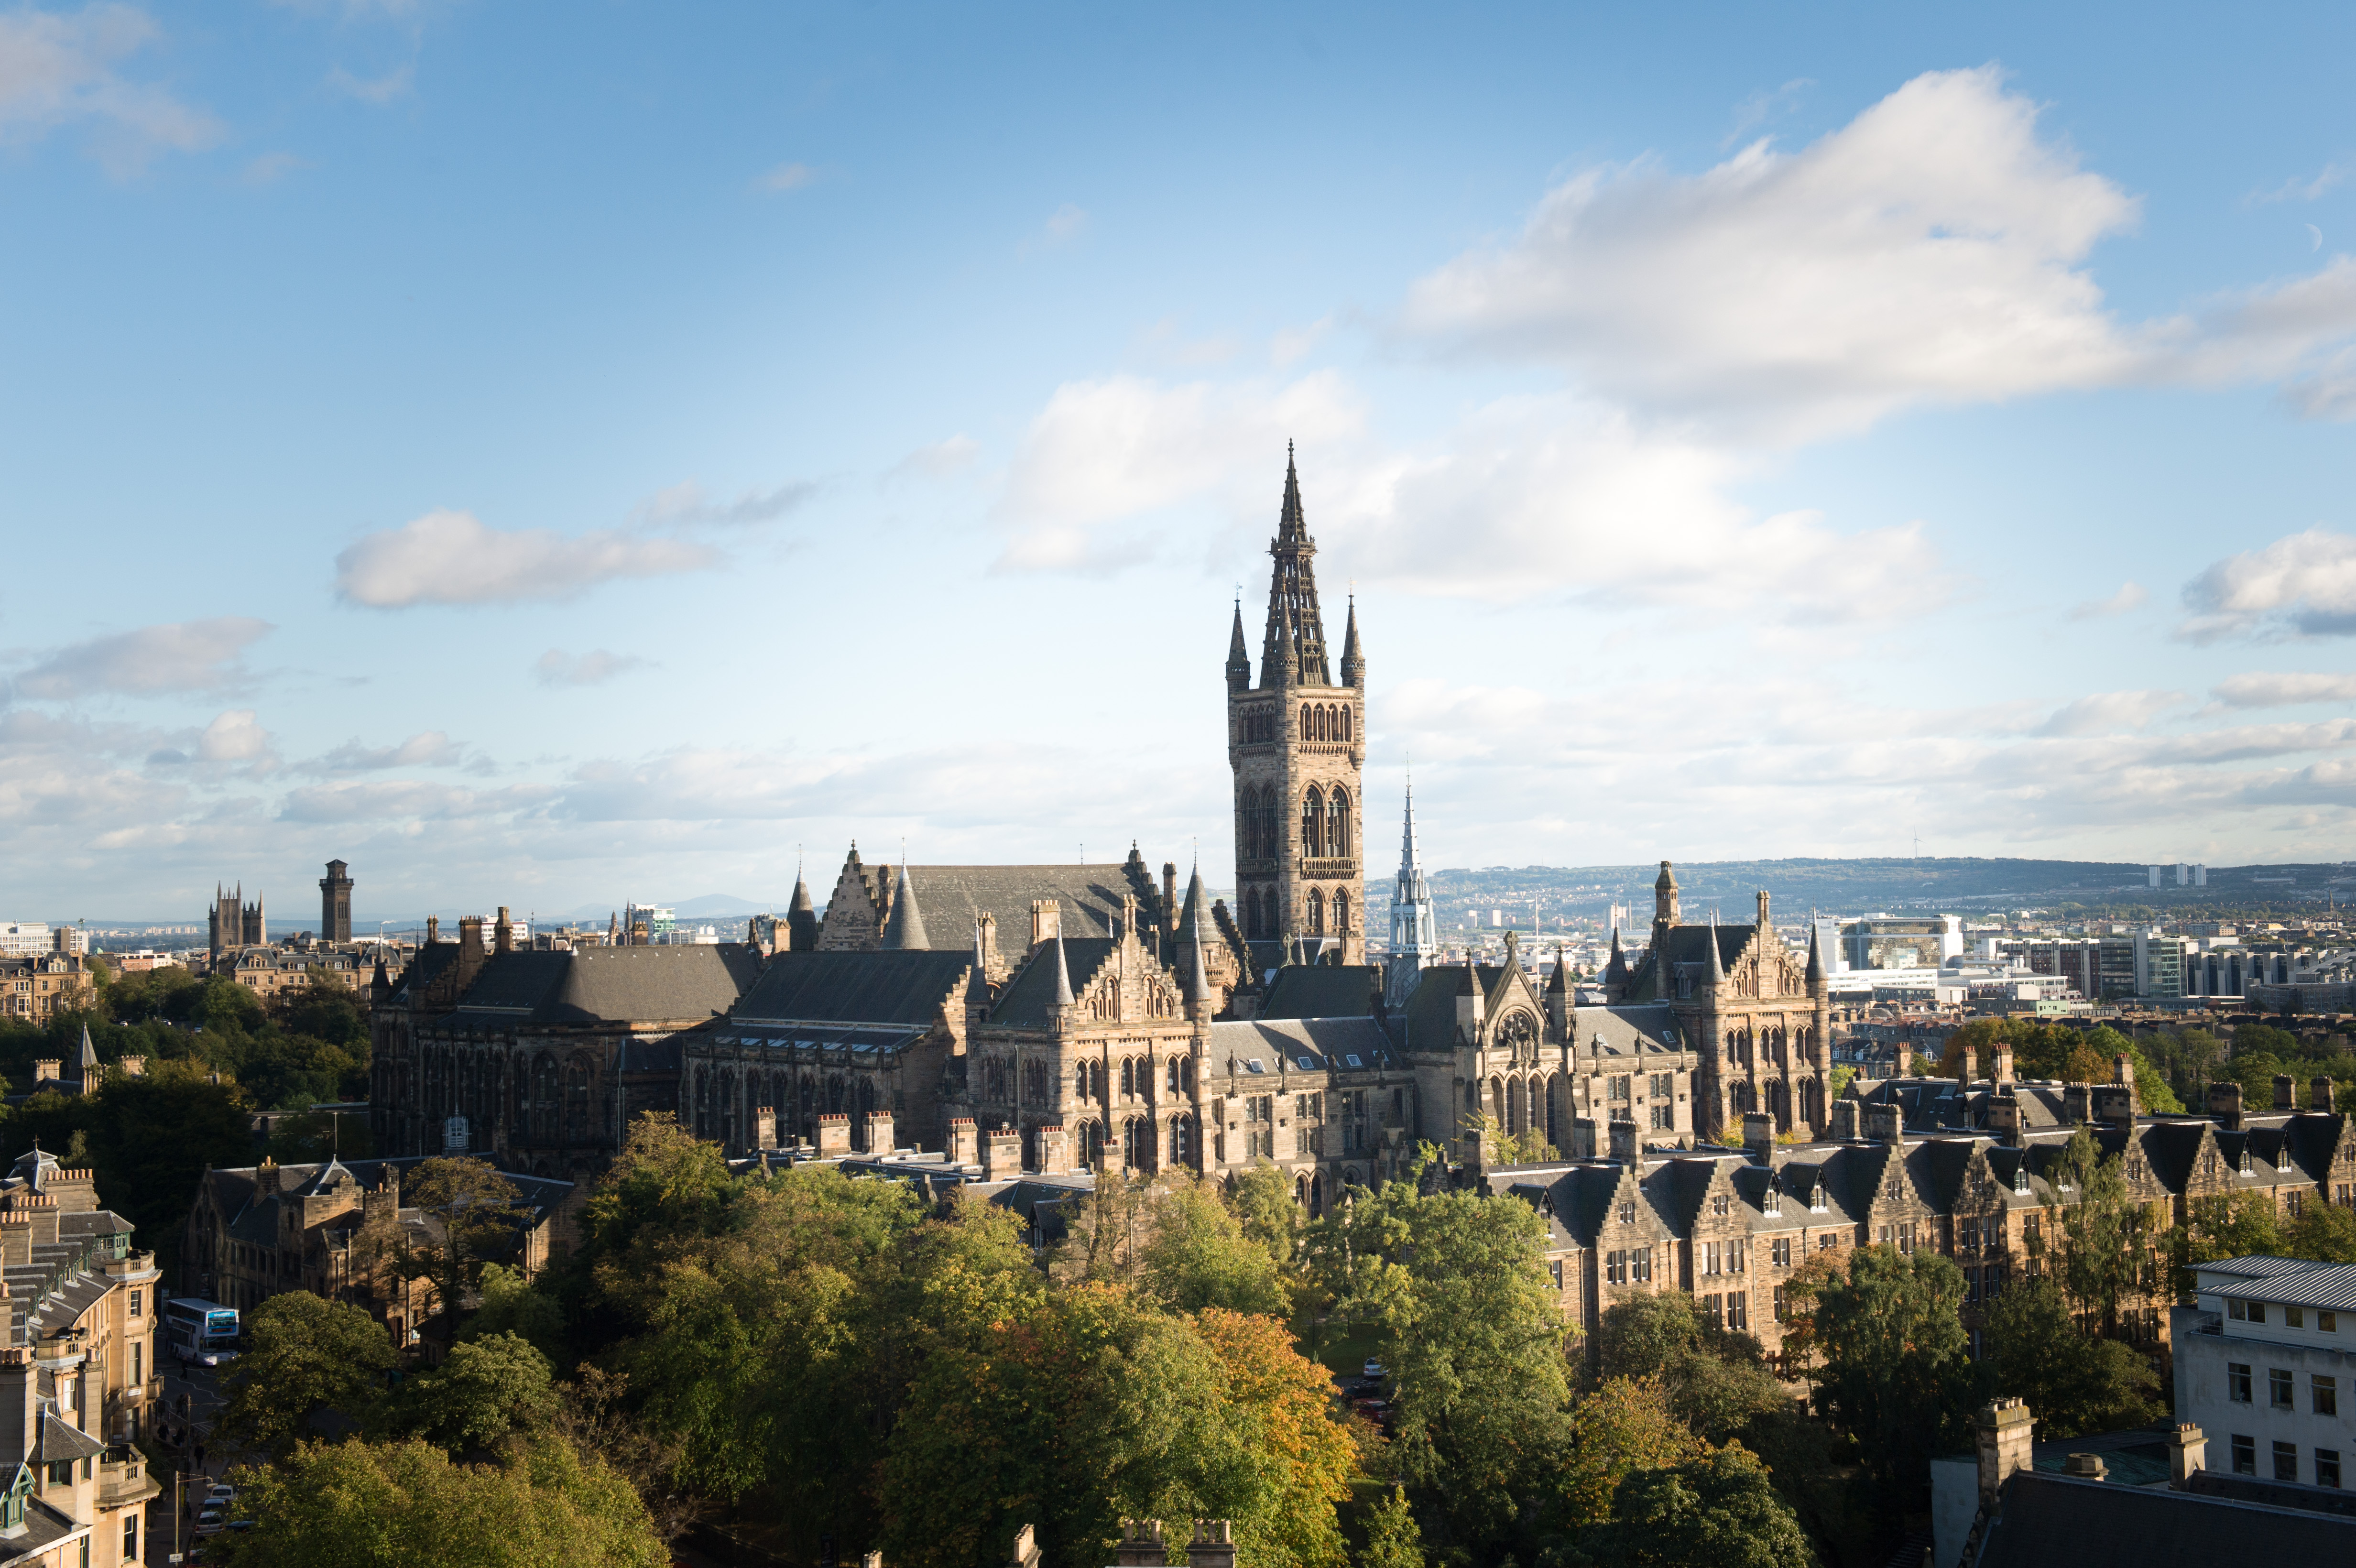
\includegraphics[keepaspectratio=true, width=\paperwidth]{../../images/background.jpg}};
    }
    \begin{frame}[plain,noframenumbering]
        \titlepage
    \end{frame}
}

\section{Finding Subgraphs}

\begin{frame}{Subgraph Isomorphism}
    \centering
    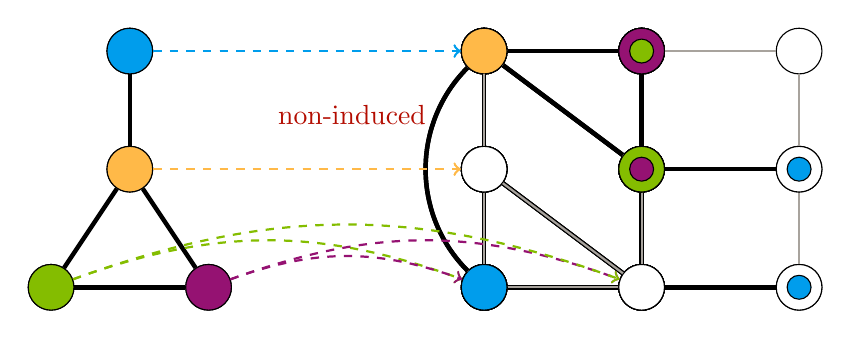
\begin{tikzpicture}
        \node <1> [draw, circle, fill=white, inner sep=4pt, font=\bfseries] (Na) at (1,  0) {\vphantom{1}};
        \node <1> [draw, circle, fill=white, inner sep=4pt, font=\bfseries] (Nb) at (1, -1.5) {\vphantom{1}};
        \node <1> [draw, circle, fill=white, inner sep=4pt, font=\bfseries] (Nc) at (0, -3) {\vphantom{1}};
        \node <1> [draw, circle, fill=white, inner sep=4pt, font=\bfseries] (Nd) at (2, -3) {\vphantom{1}};

        \node <2-> [draw, circle, fill=uofgcobalt, inner sep=4pt, font=\bfseries] (Na) at (1,  0) {\vphantom{1}};
        \node <2-> [draw, circle, fill=uofgpumpkin, inner sep=4pt, font=\bfseries] (Nb) at (1, -1.5) {\vphantom{1}};
        \node <2-> [draw, circle, fill=uofglawn, inner sep=4pt, font=\bfseries] (Nc) at (0, -3) {\vphantom{1}};
        \node <2-> [draw, circle, fill=uofgthistle, inner sep=4pt, font=\bfseries] (Nd) at (2, -3) {\vphantom{1}};

        \draw [ultra thick] (Na) -- (Nb);
        \draw [ultra thick] (Nb) -- (Nc);
        \draw [ultra thick] (Nc) -- (Nd);
        \draw [ultra thick] (Nb) -- (Nd);

        \node <1> [draw, circle, fill=white, inner sep=4pt, font=\bfseries] (N1) at (5.5,  0) {\vphantom{1}};
        \node <1> [draw, circle, fill=white, inner sep=4pt, font=\bfseries] (N2) at (7.5,  0) {\vphantom{1}};
        \node <1> [draw, circle, fill=white, inner sep=4pt, font=\bfseries] (N3) at (5.5, -1.5) {\vphantom{1}};
        \node <1> [draw, circle, fill=white, inner sep=4pt, font=\bfseries] (N4) at (7.5, -1.5) {\vphantom{1}};
        \node <1> [draw, circle, fill=white, inner sep=4pt, font=\bfseries] (N5) at (5.5, -3) {\vphantom{1}};
        \node <1> [draw, circle, fill=white, inner sep=4pt, font=\bfseries] (N6) at (7.5, -3) {\vphantom{1}};

        \node <1-6,8-> [draw, circle, fill=white, inner sep=4pt, font=\bfseries] (N7) at (9.5, -3) {\vphantom{1}};
        \node <1-4,6-> [draw, circle, fill=white, inner sep=4pt, font=\bfseries] (N8) at (9.5, -1.5) {\vphantom{1}};
        \node [draw, circle, fill=white, inner sep=4pt, font=\bfseries] (N9) at (9.5, 0) {\vphantom{1}};

        \node <2-3> [draw, circle, fill=uofgcobalt, inner sep=4pt, font=\bfseries] (N1) at (5.5,  0) {\vphantom{1}};
        \node <2-3> [draw, circle, fill=white, inner sep=4pt, font=\bfseries] (N2) at (7.5,  0) {\vphantom{1}};
        \node <2-3> [draw, circle, fill=uofgpumpkin, inner sep=4pt, font=\bfseries] (N3) at (5.5, -1.5) {\vphantom{1}};
        \node <2-3> [draw, circle, fill=white, inner sep=4pt, font=\bfseries] (N4) at (7.5, -1.5) {\vphantom{1}};
        \node <2-3> [draw, circle, fill=uofglawn, inner sep=4pt, font=\bfseries] (N5) at (5.5, -3) {\vphantom{1}};
        \node <2-3> [draw, circle, fill=uofgthistle, inner sep=4pt, font=\bfseries] (N6) at (7.5, -3) {\vphantom{1}};

        \node <4> [draw, circle, fill=uofgcobalt, inner sep=4pt, font=\bfseries] (N1) at (5.5,  0) {\vphantom{1}};
        \node <4> [draw, circle, fill=white, inner sep=4pt, font=\bfseries] (N2) at (7.5,  0) {\vphantom{1}};
        \node <4> [draw, circle, fill=uofgpumpkin, inner sep=4pt, font=\bfseries] (N3) at (5.5, -1.5) {\vphantom{1}};
        \node <4> [draw, circle, fill=white, inner sep=4pt, font=\bfseries] (N4) at (7.5, -1.5) {\vphantom{1}};
        \node <4> [draw, circle, fill=uofgthistle, inner sep=4pt, font=\bfseries] (N5) at (5.5, -3) {\vphantom{1}};
        \node <4> [draw, circle, fill=uofglawn, inner sep=4pt, font=\bfseries] (N6) at (7.5, -3) {\vphantom{1}};

        \node <5> [draw, circle, fill=uofglawn, inner sep=4pt, font=\bfseries] (N1) at (5.5,  0) {\vphantom{1}};
        \node <5> [draw, circle, fill=uofgthistle, inner sep=1pt, font=\bfseries] (N1b) at (5.5,  0) {\vphantom{1}};
        \node <5> [draw, circle, fill=uofgthistle, inner sep=4pt, font=\bfseries] (N2) at (7.5,  0) {\vphantom{1}};
        \node <5> [draw, circle, fill=uofglawn, inner sep=1pt, font=\bfseries] (N2b) at (7.5,  0) {\vphantom{1}};
        \node <5> [draw, circle, fill=white, inner sep=4pt, font=\bfseries] (N3) at (5.5, -1.5) {\vphantom{1}};
        \node <5> [draw, circle, fill=uofgpumpkin, inner sep=4pt, font=\bfseries] (N4) at (7.5, -1.5) {\vphantom{1}};
        \node <5> [draw, circle, fill=white, inner sep=4pt, font=\bfseries] (N5) at (5.5, -3) {\vphantom{1}};
        \node <5> [draw, circle, fill=white, inner sep=4pt, font=\bfseries] (N6) at (7.5, -3) {\vphantom{1}};
        \node <5> [draw, circle, fill=uofgcobalt, inner sep=1pt, font=\bfseries] (N6b) at (7.5, -3) {\vphantom{1}};
        \node <5> [draw, circle, fill=white, inner sep=4pt, font=\bfseries] (N8) at (9.5, -1.5) {\vphantom{1}};
        \node <5> [draw, circle, fill=uofgcobalt, inner sep=1pt, font=\bfseries] (N8b) at (9.5, -1.5) {\vphantom{1}};

        \node <6> [draw, circle, fill=uofgpumpkin, inner sep=4pt, font=\bfseries] (N1) at (5.5,  0) {\vphantom{1}};
        \node <6> [draw, circle, fill=uofgthistle, inner sep=4pt, font=\bfseries] (N2) at (7.5,  0) {\vphantom{1}};
        \node <6> [draw, circle, fill=uofglawn, inner sep=1pt, font=\bfseries] (N2b) at (7.5,  0) {\vphantom{1}};
        \node <6> [draw, circle, fill=uofgcobalt, inner sep=4pt, font=\bfseries] (N3) at (5.5, -1.5) {\vphantom{1}};
        \node <6> [draw, circle, fill=uofglawn, inner sep=4pt, font=\bfseries] (N4) at (7.5, -1.5) {\vphantom{1}};
        \node <6> [draw, circle, fill=uofgthistle, inner sep=1pt, font=\bfseries] (N4b) at (7.5, -1.5) {\vphantom{1}};
        \node <6> [draw, circle, fill=white, inner sep=4pt, font=\bfseries] (N5) at (5.5, -3) {\vphantom{1}};
        \node <6> [draw, circle, fill=white, inner sep=4pt, font=\bfseries] (N6) at (7.5, -3) {\vphantom{1}};

        \node <7> [draw, circle, fill=white, inner sep=4pt, font=\bfseries] (N1) at (5.5,  0) {\vphantom{1}};
        \node <7> [draw, circle, fill=white, inner sep=4pt, font=\bfseries] (N2) at (7.5,  0) {\vphantom{1}};
        \node <7> [draw, circle, fill=uofgthistle, inner sep=4pt, font=\bfseries] (N3) at (5.5, -1.5) {\vphantom{1}};
        \node <7> [draw, circle, fill=uofglawn, inner sep=1pt, font=\bfseries] (N3b) at (5.5, -1.5) {\vphantom{1}};
        \node <7> [draw, circle, fill=white, inner sep=4pt, font=\bfseries] (N4) at (7.5, -1.5) {\vphantom{1}};
        \node <7> [draw, circle, fill=uofgcobalt, inner sep=1pt, font=\bfseries] (N4b) at (7.5, -1.5) {\vphantom{1}};
        \node <7> [draw, circle, fill=uofglawn, inner sep=4pt, font=\bfseries] (N5) at (5.5, -3) {\vphantom{1}};
        \node <7> [draw, circle, fill=uofgthistle, inner sep=1pt, font=\bfseries] (N5b) at (5.5, -3) {\vphantom{1}};
        \node <7> [draw, circle, fill=uofgpumpkin, inner sep=4pt, font=\bfseries] (N6) at (7.5, -3) {\vphantom{1}};
        \node <7> [draw, circle, fill=white, inner sep=4pt, font=\bfseries] (N7) at (9.5, -3) {\vphantom{1}};
        \node <7> [draw, circle, fill=uofgcobalt, inner sep=1pt, font=\bfseries] (N7b) at (9.5, -3) {\vphantom{1}};

        \node <8> [draw, circle, fill=uofgcobalt, inner sep=4pt, font=\bfseries] (N1) at (5.5,  0) {\vphantom{1}};
        \node <8> [draw, circle, fill=white, inner sep=4pt, font=\bfseries] (N2) at (7.5,  0) {\vphantom{1}};
        \node <8> [draw, circle, fill=uofglawn, inner sep=4pt, font=\bfseries] (N3) at (5.5, -1.5) {\vphantom{1}};
        \node <8> [draw, circle, fill=uofgthistle, inner sep=1pt, font=\bfseries] (N3b) at (5.5, -1.5) {\vphantom{1}};
        \node <8> [draw, circle, fill=white, inner sep=4pt, font=\bfseries] (N4) at (7.5, -1.5) {\vphantom{1}};
        \node <8> [draw, circle, fill=uofgpumpkin, inner sep=4pt, font=\bfseries] (N5) at (5.5, -3) {\vphantom{1}};
        \node <8> [draw, circle, fill=uofgthistle, inner sep=4pt, font=\bfseries] (N6) at (7.5, -3) {\vphantom{1}};
        \node <8> [draw, circle, fill=uofglawn, inner sep=1pt, font=\bfseries] (N6b) at (7.5, -3) {\vphantom{1}};

        \node <9-> [draw, circle, fill=uofgpumpkin, inner sep=4pt, font=\bfseries] (N1) at (5.5,  0) {\vphantom{1}};
        \node <9-> [draw, circle, fill=uofgthistle, inner sep=4pt, font=\bfseries] (N2) at (7.5,  0) {\vphantom{1}};
        \node <9-> [draw, circle, fill=uofglawn, inner sep=1pt, font=\bfseries] (N2b) at (7.5,  0) {\vphantom{1}};
        \node <9-> [draw, circle, fill=white, inner sep=4pt, font=\bfseries] (N3) at (5.5, -1.5) {\vphantom{1}};
        \node <9-> [draw, circle, fill=uofglawn, inner sep=4pt, font=\bfseries] (N4) at (7.5, -1.5) {\vphantom{1}};
        \node <9-> [draw, circle, fill=uofgthistle, inner sep=1pt, font=\bfseries] (N4b) at (7.5, -1.5) {\vphantom{1}};
        \node <9-> [draw, circle, fill=uofgcobalt, inner sep=4pt, font=\bfseries] (N5) at (5.5, -3) {\vphantom{1}};
        \node <9-> [draw, circle, fill=white, inner sep=4pt, font=\bfseries] (N6) at (7.5, -3) {\vphantom{1}};

        \draw <1> [thick, color=uofgsandstone!50] (N1) -- (N2);
        \draw <1> [thick, color=uofgsandstone!50] (N1) -- (N3);
        \draw <1> [thick, color=uofgsandstone!50] (N1) -- (N4);
        \draw <1> [thick, color=uofgsandstone!50] (N2) -- (N4);
        \draw <1> [thick, color=uofgsandstone!50] (N3) -- (N5);
        \draw <1> [thick, color=uofgsandstone!50] (N3) -- (N6);
        \draw <1> [thick, color=uofgsandstone!50] (N4) -- (N6);
        \draw <1> [thick, color=uofgsandstone!50] (N5) -- (N6);
        \draw <1> [thick, color=uofgsandstone!50] (N1) to [in=135, out=225] (N5);

        \draw <2-4> [thick, color=uofgsandstone!50] (N1) -- (N2);
        \draw <2-4> [ultra thick] (N1) -- (N3);
        \draw <2-4> [thick, color=uofgsandstone!50] (N1) -- (N4);
        \draw <2-4> [thick, color=uofgsandstone!50] (N2) -- (N4);
        \draw <2-4> [ultra thick] (N3) -- (N5);
        \draw <2-4> [ultra thick] (N3) -- (N6);
        \draw <2-4> [thick, color=uofgsandstone!50] (N4) -- (N6);
        \draw <2-4> [ultra thick] (N5) -- (N6);
        \draw <2> [thick, color=uofgsandstone!50] (N1) to [in=135, out=225] (N5);
        \draw <3> [thick, color=uofgpillarbox] (N1) to [in=135, out=225] node [near start, left] { non-induced } (N5);
        \draw <4> [thick, color=uofgsandstone!50] (N1) to [in=135, out=225] (N5);

        \draw <5> [ultra thick] (N1) -- (N2);
        \draw <5> [thick, color=uofgsandstone!50] (N1) -- (N3);
        \draw <5> [ultra thick] (N1) -- (N4);
        \draw <5> [ultra thick] (N2) -- (N4);
        \draw <5> [thick, color=uofgsandstone!50] (N3) -- (N5);
        \draw <5> [thick, color=uofgsandstone!50] (N3) -- (N6);
        \draw <5> [ultra thick] (N4) -- (N6);
        \draw <5> [thick, color=uofgsandstone!50] (N5) -- (N6);
        \draw <5> [thick, color=uofgsandstone!50] (N1) to [in=135, out=225] (N5);

        \draw <6> [ultra thick] (N1) -- (N2);
        \draw <6> [ultra thick] (N1) -- (N3);
        \draw <6> [ultra thick] (N1) -- (N4);
        \draw <6> [ultra thick] (N2) -- (N4);
        \draw <6> [thick, color=uofgsandstone!50] (N3) -- (N5);
        \draw <6> [thick, color=uofgsandstone!50] (N3) -- (N6);
        \draw <6> [thick, color=uofgsandstone!50] (N4) -- (N6);
        \draw <6> [thick, color=uofgsandstone!50] (N5) -- (N6);
        \draw <6> [thick, color=uofgsandstone!50] (N1) to [in=135, out=225] (N5);

        \draw <7> [thick, color=uofgsandstone!50] (N1) -- (N2);
        \draw <7> [thick, color=uofgsandstone!50] (N1) -- (N3);
        \draw <7> [thick, color=uofgsandstone!50] (N1) -- (N4);
        \draw <7> [thick, color=uofgsandstone!50] (N2) -- (N4);
        \draw <7> [ultra thick] (N3) -- (N5);
        \draw <7> [ultra thick] (N3) -- (N6);
        \draw <7> [ultra thick] (N4) -- (N6);
        \draw <7> [ultra thick] (N5) -- (N6);
        \draw <7> [thick, color=uofgsandstone!50] (N1) to [in=135, out=225] (N5);

        \draw <8> [thick, color=uofgsandstone!50] (N1) -- (N2);
        \draw <8> [thick, color=uofgsandstone!50] (N1) -- (N3);
        \draw <8> [thick, color=uofgsandstone!50] (N1) -- (N4);
        \draw <8> [thick, color=uofgsandstone!50] (N2) -- (N4);
        \draw <8> [ultra thick] (N3) -- (N5);
        \draw <8> [ultra thick] (N3) -- (N6);
        \draw <8> [thick, color=uofgsandstone!50] (N4) -- (N6);
        \draw <8> [ultra thick] (N5) -- (N6);
        \draw <8> [ultra thick] (N1) to [in=135, out=225] (N5);

        \draw <9-> [ultra thick] (N1) -- (N2);
        \draw <9-> [thick, color=uofgsandstone!50] (N1) -- (N3);
        \draw <9-> [ultra thick] (N1) -- (N4);
        \draw <9-> [ultra thick] (N2) -- (N4);
        \draw <9-> [thick, color=uofgsandstone!50] (N3) -- (N5);
        \draw <9-> [thick, color=uofgsandstone!50] (N3) -- (N6);
        \draw <9-> [thick, color=uofgsandstone!50] (N4) -- (N6);
        \draw <9-> [thick, color=uofgsandstone!50] (N5) -- (N6);
        \draw <9-> [ultra thick] (N1) to [in=135, out=225] (N5);

        \draw <2-3> [thick, dashed, color=uofgcobalt, arrows=->] (Na) to (N1);
        \draw <2-3> [thick, dashed, color=uofgpumpkin, arrows=->] (Nb) to (N3);
        \draw <2-3> [thick, dashed, color=uofglawn, arrows=->] (Nc) to [out=20, in=160] (N5);
        \draw <2-3> [thick, dashed, color=uofgthistle, arrows=->] (Nd) to [out=20, in=160] (N6);

        \draw <4> [thick, dashed, color=uofgcobalt, arrows=->] (Na) to (N1);
        \draw <4> [thick, dashed, color=uofgpumpkin, arrows=->] (Nb) to (N3);
        \draw <4> [thick, dashed, color=uofglawn, arrows=->] (Nc) to [out=20, in=160] (N6);
        \draw <4> [thick, dashed, color=uofgthistle, arrows=->] (Nd) to [out=20, in=160] (N5);

        \draw [thick, color=uofgsandstone!50] (N7) -- (N8);
        \draw [thick, color=uofgsandstone!50] (N8) -- (N9);
        \draw [thick, color=uofgsandstone!50] (N2) -- (N9);
        \draw <1-4,6-> [thick, color=uofgsandstone!50] (N4) -- (N8);
        \draw <5> [ultra thick] (N4) -- (N8);
        \draw <1-6,8-> [thick, color=uofgsandstone!50] (N6) -- (N7);
        \draw <7> [ultra thick] (N6) -- (N7);
    \end{tikzpicture}

    \uncover<10->{

        \bigskip

        How many did I miss?
    }
\end{frame}

\begin{frame}{The Maximum Clique Problem}
    \begin{center}
    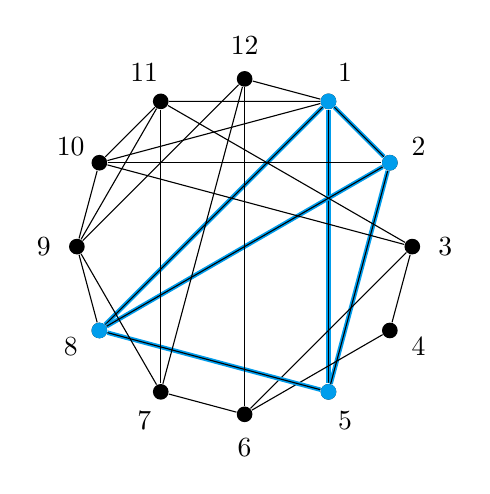
\begin{tikzpicture}
        \begin{scope}[scale=1.5]
        \newcount \myc
        \foreach \n in {3, 4, 6, 7, 9, 10, 11, 12}{
            \myc=\n \advance\myc by -1 \multiply\myc by -360 \divide\myc by 12 \advance\myc by 60
            \node[anchor=center] (L\n) at (\the\myc:1.7) {\n};
            \node[anchor=center, circle, fill=black, inner sep=2pt] (N\n) at (\the\myc:1.42) {};
        }
        \foreach \n in {1, 2, 5, 8}{
            \myc=\n \advance\myc by -1 \multiply\myc by -360 \divide\myc by 12 \advance\myc by 60
            \node[anchor=center] (L\n) at (\the\myc:1.7) {\n};
            \node<1>[anchor=center, circle, fill=black, inner sep=2pt] (N\n) at (\the\myc:1.42) {};
            \node<2>[anchor=center, circle, fill=uofgcobalt, inner sep=2pt] (N\n) at (\the\myc:1.42) {};
        }
        \draw <2> [ultra thick, color=uofgcobalt] (N1) -- (N2);
        \draw <2> [ultra thick, color=uofgcobalt] (N1) -- (N5);
        \draw <2> [ultra thick, color=uofgcobalt] (N1) -- (N8);
        \draw <1> (N1) -- (N2);
        \draw <1> (N1) -- (N5);
        \draw <1> (N1) -- (N8);
        \draw (N1) -- (N10);
        \draw (N1) -- (N11);
        \draw (N1) -- (N12);
        \draw <2> [ultra thick, color=uofgcobalt] (N2) -- (N5);
        \draw <2> [ultra thick, color=uofgcobalt] (N2) -- (N8);
        \draw <1> (N2) -- (N5);
        \draw <1> (N2) -- (N8);
        \draw (N2) -- (N10);
        \draw (N3) -- (N4);
        \draw (N3) -- (N6);
        \draw (N3) -- (N10);
        \draw (N3) -- (N11);
        \draw (N4) -- (N6);
        \draw <2> [ultra thick, color=uofgcobalt] (N5) -- (N8);
        \draw <1> (N5) -- (N8);
        \draw (N6) -- (N7);
        \draw (N6) -- (N12);
        \draw (N7) -- (N9);
        \draw (N7) -- (N11);
        \draw (N7) -- (N12);
        \draw (N8) -- (N9);
        \draw (N9) -- (N10);
        \draw (N9) -- (N11);
        \draw (N9) -- (N12);
        \draw (N10) -- (N11);
    \end{scope}
    \end{tikzpicture}
    \end{center}
\end{frame}

\begin{frame}{Maximum Common Subgraph}
    \only<1>{\centering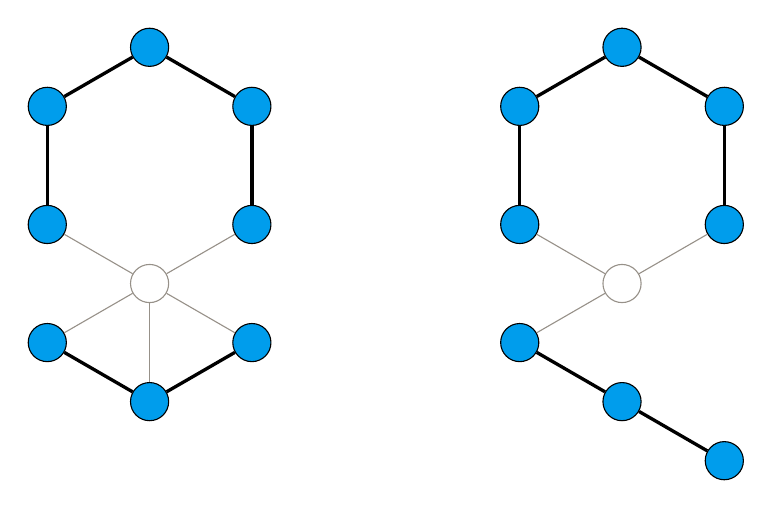
\begin{tikzpicture}
        \begin{scope}
            \node[draw, circle, fill=uofgcobalt, inner sep=2pt, font=\normalsize] (M1) at (90:1.5) {\phantom{0}};
            \node[draw, circle, fill=uofgcobalt, inner sep=2pt, font=\normalsize] (M2) at (150:1.5) {\phantom{0}};
            \node[draw, circle, fill=uofgcobalt, inner sep=2pt, font=\normalsize] (M3) at (30:1.5) {\phantom{0}};
            \node[draw, circle, fill=uofgcobalt, inner sep=2pt, font=\normalsize] (M4) at (210:1.5) {\phantom{0}};
            \node[draw, circle, fill=uofgcobalt, inner sep=2pt, font=\normalsize] (M5) at (330:1.5) {\phantom{0}};
            \node[draw, circle, draw=uofgsandstone!60, fill=white, inner sep=2pt, font=\normalsize] (M6) at (270:1.5) {\phantom{0}};
            \node[draw, circle, fill=uofgcobalt, inner sep=2pt, font=\normalsize] (M7) at ($(210:1.5) + (M6)$) {\phantom{0}};
            \node[draw, circle, fill=uofgcobalt, inner sep=2pt, font=\normalsize] (M8) at ($(330:1.5) + (M6)$) {\phantom{0}};
            \node[draw, circle, fill=uofgcobalt, inner sep=2pt, font=\normalsize] (M9) at ($(270:1.5) + (M6)$) {\phantom{0}};

            \draw [very thick] (M1) -- (M2);
            \draw [very thick] (M2) -- (M4);
            \draw [very thick] (M3) -- (M5);
            \draw [color=uofgsandstone!60] (M4) -- (M6);
            \draw [color=uofgsandstone!60] (M5) -- (M6);
            \draw [very thick] (M3) -- (M1);
            \draw [color=uofgsandstone!60] (M6) -- (M7);
            \draw [color=uofgsandstone!60] (M6) -- (M8);
            \draw [color=uofgsandstone!60] (M6) -- (M9);
            \draw [very thick] (M7) -- (M9);
            \draw [very thick] (M8) -- (M9);
        \end{scope}

        \begin{scope}[xshift=6cm]
            \node[draw, circle, fill=uofgcobalt, inner sep=2pt, font=\normalsize] (M1) at (90:1.5) {\phantom{0}};
            \node[draw, circle, fill=uofgcobalt, inner sep=2pt, font=\normalsize] (M2) at (150:1.5) {\phantom{0}};
            \node[draw, circle, fill=uofgcobalt, inner sep=2pt, font=\normalsize] (M3) at (30:1.5) {\phantom{0}};
            \node[draw, circle, fill=uofgcobalt, inner sep=2pt, font=\normalsize] (M4) at (210:1.5) {\phantom{0}};
            \node[draw, circle, fill=uofgcobalt, inner sep=2pt, font=\normalsize] (M5) at (330:1.5) {\phantom{0}};
            \node[draw, circle, draw=uofgsandstone!60, fill=white, inner sep=2pt, font=\normalsize] (M6) at (270:1.5) {\phantom{0}};
            \node[draw, circle, fill=uofgcobalt, inner sep=2pt, font=\normalsize] (M7) at ($(210:1.5) + (M6)$) {\phantom{0}};
            \node[draw, circle, fill=uofgcobalt, inner sep=2pt, font=\normalsize] (M8) at ($(270:1.5) + (M6)$) {\phantom{0}};
            \node[draw, circle, fill=uofgcobalt, inner sep=2pt, font=\normalsize] (M9) at ($(330:1.5) + (M8)$) {\phantom{0}};

            \draw [very thick] (M1) -- (M2);
            \draw [very thick] (M2) -- (M4);
            \draw [very thick] (M3) -- (M5);
            \draw [color=uofgsandstone!60] (M4) -- (M6);
            \draw [color=uofgsandstone!60] (M5) -- (M6);
            \draw [very thick] (M3) -- (M1);
            \draw [color=uofgsandstone!60] (M6) -- (M7);
            \draw [very thick] (M7) -- (M8);
            \draw [very thick] (M8) -- (M9);
        \end{scope}
    \end{tikzpicture}}\only<2>{\centering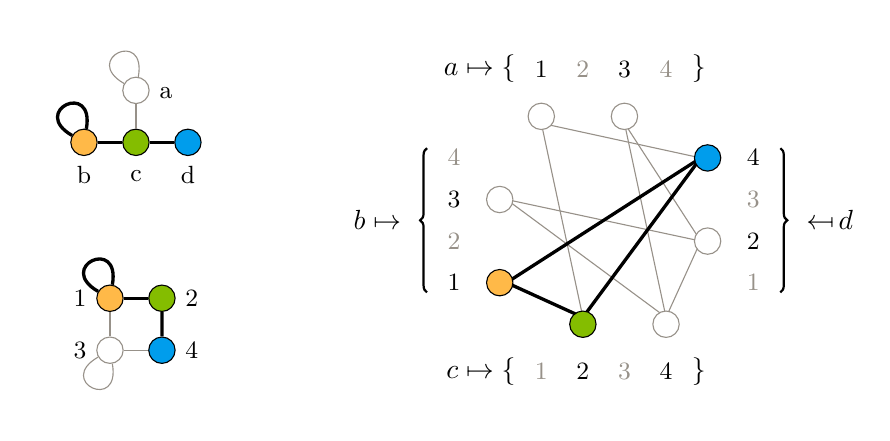
\begin{tikzpicture}[scale=0.33]%{{{
        \begin{scope}
            \node[draw, circle, fill=white, draw=uofgsandstone!60, inner sep=0.5pt, font=\normalsize] (Ma) at (2, 8) {\phantom{0}};
            \node[draw, circle, fill=uofgpumpkin, inner sep=0.5pt, font=\normalsize] (Mb) at (0, 6) {\phantom{0}};
            \node[draw, circle, fill=uofglawn, inner sep=0.5pt, font=\normalsize] (Mc) at (2, 6) {\phantom{0}};
            \node[draw, circle, fill=uofgcobalt, inner sep=0.5pt, font=\normalsize] (Md) at (4, 6) {\phantom{0}};

            \node [right = 0 of Ma, font=\small] { \vphantom{0}a };
            \node [below = 0 of Mb, font=\small] { \vphantom{0}b };
            \node [below = 0 of Mc, font=\small] { \vphantom{0}c };
            \node [below = 0 of Md, font=\small] { \vphantom{0}d };

            \draw [very thick] (Mb) -- (Mc);
            \draw [very thick] (Mc) -- (Md);
            \draw [color=uofgsandstone!60] (Ma) -- (Mc);
            \draw [color=uofgsandstone!60] (Ma) to [out=150, in=80, looseness=8] (Ma);
            \draw [very thick] (Mb) to [out=150, in=80, looseness=8] (Mb);
        \end{scope}

        \begin{scope}[yshift=-2cm]
            \node[draw, circle, fill=uofgpumpkin, inner sep=0.5pt, font=\normalsize] (M1) at (1, 2) {\phantom{0}};
            \node[draw, circle, fill=uofglawn, inner sep=0.5pt, font=\normalsize] (M2) at (3, 2) {\phantom{0}};
            \node[draw, circle, fill=white, draw=uofgsandstone!60, inner sep=0.5pt, font=\normalsize] (M3) at (1, 0) {\phantom{0}};
            \node[draw, circle, fill=uofgcobalt, inner sep=0.5pt, font=\normalsize] (M4) at (3, 0) {\phantom{0}};

            \node [left = 0 of M1, font=\small] { \vphantom{0}1 };
            \node [right = 0 of M2, font=\small] { \vphantom{0}2 };
            \node [left = 0 of M3, font=\small] { \vphantom{0}3 };
            \node [right = 0 of M4, font=\small] { \vphantom{0}4 };

            \draw [very thick] (M1) -- (M2);
            \draw [very thick] (M2) -- (M4);
            \draw [color=uofgsandstone!60] (M3) -- (M4);
            \draw [color=uofgsandstone!60] (M1) -- (M3);

            \draw [color=uofgsandstone!60] (M3) to [out=280, in=210, looseness=8] (M3);
            \draw [very thick] (M1) to [out=150, in=80, looseness=8] (M1);
        \end{scope}

        \begin{scope}[xshift=15cm, yshift=-2cm]
            \node[draw, circle, fill=white, draw=uofgsandstone!60, inner sep=0.5pt, font=\normalsize] (Ma1) at (2.6, 9) {\phantom{0}};
            \node[draw, circle, fill=white, draw=white, inner sep=0.5pt, font=\normalsize] (Ma2) at (4.2, 9) {\phantom{0}};
            \node[draw, circle, fill=white, draw=uofgsandstone!60, inner sep=0.5pt, font=\normalsize] (Ma3) at (5.8, 9) {\phantom{0}};
            \node[draw, circle, fill=white, draw=white, inner sep=0.5pt, font=\normalsize] (Ma4) at (7.4, 9) {\phantom{0}};
            \node (La1) [above = 0.2cm of Ma1, font=\small] { \vphantom{0}1 };
            \node (La2) [above = 0.2cm of Ma2, font=\small, color=uofgsandstone!60] { \vphantom{0}2 };
            \node (La3) [above = 0.2cm of Ma3, font=\small] { \vphantom{0}3 };
            \node (La4) [above = 0.2cm of Ma4, font=\small, color=uofgsandstone!60] { \vphantom{0}4 };

            \node [left=0 of La1] { $a \mapsto \{$ };
            \node [right=0 of La4] { $\}$ };

            \node[draw, circle, fill=uofgpumpkin, inner sep=0.5pt, font=\normalsize] (Mb1) at (1, 2.6) {\phantom{0}};
            \node[draw, circle, fill=white, draw=white, inner sep=0.5pt, font=\normalsize] (Mb2) at (1, 4.2) {\phantom{0}};
            \node[draw, circle, fill=white, draw=uofgsandstone!60, inner sep=0.5pt, font=\normalsize] (Mb3) at (1, 5.8) {\phantom{0}};
            \node[draw, circle, fill=white, draw=white, inner sep=0.5pt, font=\normalsize] (Mb4) at (1, 7.4) {\phantom{0}};
            \node [left = 0.2cm of Mb1, font=\small] { \vphantom{0}1 };
            \node [left = 0.2cm of Mb2, font=\small, color=uofgsandstone!60] { \vphantom{0}2 };
            \node [left = 0.2cm of Mb3, font=\small] { \vphantom{0}3 };
            \node [left = 0.2cm of Mb4, font=\small, color=uofgsandstone!60] { \vphantom{0}4 };

            \draw [decorate, decoration={brace, raise=0.8cm}, thick] (Mb1.south west) -- (Mb4.north west) node [midway, left=1cm] { $b \mapsto$ };

            \node[draw, circle, fill=white, draw=white, inner sep=0.5pt, font=\normalsize] (Mc1) at (2.6, 1) {\phantom{0}};
            \node[draw, circle, fill=uofglawn, inner sep=0.5pt, font=\normalsize] (Mc2) at (4.2, 1) {\phantom{0}};
            \node[draw, circle, fill=white, draw=white, inner sep=0.5pt, font=\normalsize] (Mc3) at (5.8, 1) {\phantom{0}};
            \node[draw, circle, fill=white, draw=uofgsandstone!60, inner sep=0.5pt, font=\normalsize] (Mc4) at (7.4, 1) {\phantom{0}};
            \node (Lc1) [below = 0.2cm of Mc1, font=\small, color=uofgsandstone!60] { \vphantom{0}1 };
            \node (Lc2) [below = 0.2cm of Mc2, font=\small] { \vphantom{0}2 };
            \node (Lc3) [below = 0.2cm of Mc3, font=\small, color=uofgsandstone!60] { \vphantom{0}3 };
            \node (Lc4) [below = 0.2cm of Mc4, font=\small] { \vphantom{0}4 };

            \node [left=0 of Lc1] { $c \mapsto \{$ };
            \node [right=0 of Lc4] { $\}$ };

            \node[draw, circle, fill=white, draw=white, inner sep=0.5pt, font=\normalsize] (Md1) at (9, 2.6) {\phantom{0}};
            \node[draw, circle, fill=white, draw=uofgsandstone!60, inner sep=0.5pt, font=\normalsize] (Md2) at (9, 4.2) {\phantom{0}};
            \node[draw, circle, fill=white, draw=white, inner sep=0.5pt, font=\normalsize] (Md3) at (9, 5.8) {\phantom{0}};
            \node[draw, circle, fill=uofgcobalt, inner sep=0.5pt, font=\normalsize] (Md4) at (9, 7.4) {\phantom{0}};
            \node [right = 0.2cm of Md1, font=\small, color=uofgsandstone!60] { \vphantom{0}1 };
            \node [right = 0.2cm of Md2, font=\small] { \vphantom{0}2 };
            \node [right = 0.2cm of Md3, font=\small, color=uofgsandstone!60] { \vphantom{0}3 };
            \node [right = 0.2cm of Md4, font=\small] { \vphantom{0}4 };

            \draw [decorate, decoration={brace, raise=0.8cm}, thick] (Md4.north east) -- (Md1.south east) node [midway, right=1cm] { $\reflectbox{\ensuremath{\mapsto}}\, d$ };

            \begin{scope}[on background layer]
                \draw [draw=uofgsandstone!60] ($(Ma1.south)!0.5!(Ma1)$) -- ($(Md4.west)!0.5!(Md4)$);
                \draw [draw=uofgsandstone!60] ($(Ma1.south)!0.5!(Ma1)$) -- ($(Mc2.north)!0.5!(Mc2)$);
                \draw [draw=uofgsandstone!60] ($(Ma3.south)!0.5!(Ma3)$) -- ($(Mc4.north)!0.5!(Mc4)$);
                \draw [draw=uofgsandstone!60] ($(Mb3.east)!0.5!(Mb3)$) -- ($(Mc4.north)!0.5!(Mc4)$);
                \draw [draw=uofgsandstone!60] ($(Md2.west)!0.5!(Md2)$) -- ($(Mc4.north)!0.5!(Mc4)$);
                \draw [draw=uofgsandstone!60] ($(Md2.west)!0.5!(Md2)$) -- ($(Ma3.south)!0.5!(Ma3)$);
                \draw [draw=uofgsandstone!60] ($(Md2.west)!0.5!(Md2)$) -- ($(Mb3.east)!0.5!(Mb3)$);
                \draw [very thick] ($(Mb1.east)!0.5!(Mb1)$) -- ($(Mc2.north)!0.5!(Mc2)$);
                \draw [very thick] ($(Mb1.east)!0.5!(Mb1)$) -- ($(Md4.west)!0.5!(Md4)$);
                \draw [very thick] ($(Mc2.north)!0.5!(Mc2)$) -- ($(Md4.west)!0.5!(Md4)$);
        \end{scope}
        \end{scope}

    \end{tikzpicture}}
\end{frame}

\begin{frame}{Maximum Common Connected Subgraph?}
    \centering
    \only<1>{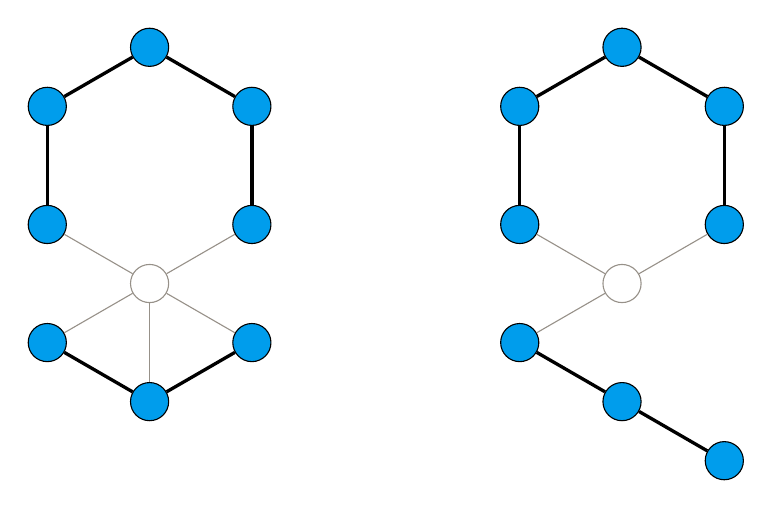
\begin{tikzpicture}
        \begin{scope}
            \node[draw, circle, fill=uofgcobalt, inner sep=2pt, font=\normalsize] (M1) at (90:1.5) {\phantom{0}};
            \node[draw, circle, fill=uofgcobalt, inner sep=2pt, font=\normalsize] (M2) at (150:1.5) {\phantom{0}};
            \node[draw, circle, fill=uofgcobalt, inner sep=2pt, font=\normalsize] (M3) at (30:1.5) {\phantom{0}};
            \node[draw, circle, fill=uofgcobalt, inner sep=2pt, font=\normalsize] (M4) at (210:1.5) {\phantom{0}};
            \node[draw, circle, fill=uofgcobalt, inner sep=2pt, font=\normalsize] (M5) at (330:1.5) {\phantom{0}};
            \node[draw, circle, draw=uofgsandstone!60, fill=white, inner sep=2pt, font=\normalsize] (M6) at (270:1.5) {\phantom{0}};
            \node[draw, circle, fill=uofgcobalt, inner sep=2pt, font=\normalsize] (M7) at ($(210:1.5) + (M6)$) {\phantom{0}};
            \node[draw, circle, fill=uofgcobalt, inner sep=2pt, font=\normalsize] (M8) at ($(330:1.5) + (M6)$) {\phantom{0}};
            \node[draw, circle, fill=uofgcobalt, inner sep=2pt, font=\normalsize] (M9) at ($(270:1.5) + (M6)$) {\phantom{0}};

            \draw [very thick] (M1) -- (M2);
            \draw [very thick] (M2) -- (M4);
            \draw [very thick] (M3) -- (M5);
            \draw [color=uofgsandstone!60] (M4) -- (M6);
            \draw [color=uofgsandstone!60] (M5) -- (M6);
            \draw [very thick] (M3) -- (M1);
            \draw [color=uofgsandstone!60] (M6) -- (M7);
            \draw [color=uofgsandstone!60] (M6) -- (M8);
            \draw [color=uofgsandstone!60] (M6) -- (M9);
            \draw [very thick] (M7) -- (M9);
            \draw [very thick] (M8) -- (M9);
        \end{scope}

        \begin{scope}[xshift=6cm]
            \node[draw, circle, fill=uofgcobalt, inner sep=2pt, font=\normalsize] (M1) at (90:1.5) {\phantom{0}};
            \node[draw, circle, fill=uofgcobalt, inner sep=2pt, font=\normalsize] (M2) at (150:1.5) {\phantom{0}};
            \node[draw, circle, fill=uofgcobalt, inner sep=2pt, font=\normalsize] (M3) at (30:1.5) {\phantom{0}};
            \node[draw, circle, fill=uofgcobalt, inner sep=2pt, font=\normalsize] (M4) at (210:1.5) {\phantom{0}};
            \node[draw, circle, fill=uofgcobalt, inner sep=2pt, font=\normalsize] (M5) at (330:1.5) {\phantom{0}};
            \node[draw, circle, draw=uofgsandstone!60, fill=white, inner sep=2pt, font=\normalsize] (M6) at (270:1.5) {\phantom{0}};
            \node[draw, circle, fill=uofgcobalt, inner sep=2pt, font=\normalsize] (M7) at ($(210:1.5) + (M6)$) {\phantom{0}};
            \node[draw, circle, fill=uofgcobalt, inner sep=2pt, font=\normalsize] (M8) at ($(270:1.5) + (M6)$) {\phantom{0}};
            \node[draw, circle, fill=uofgcobalt, inner sep=2pt, font=\normalsize] (M9) at ($(330:1.5) + (M8)$) {\phantom{0}};

            \draw [very thick] (M1) -- (M2);
            \draw [very thick] (M2) -- (M4);
            \draw [very thick] (M3) -- (M5);
            \draw [color=uofgsandstone!60] (M4) -- (M6);
            \draw [color=uofgsandstone!60] (M5) -- (M6);
            \draw [very thick] (M3) -- (M1);
            \draw [color=uofgsandstone!60] (M6) -- (M7);
            \draw [very thick] (M7) -- (M8);
            \draw [very thick] (M8) -- (M9);
        \end{scope}
    \end{tikzpicture}}\only<2>{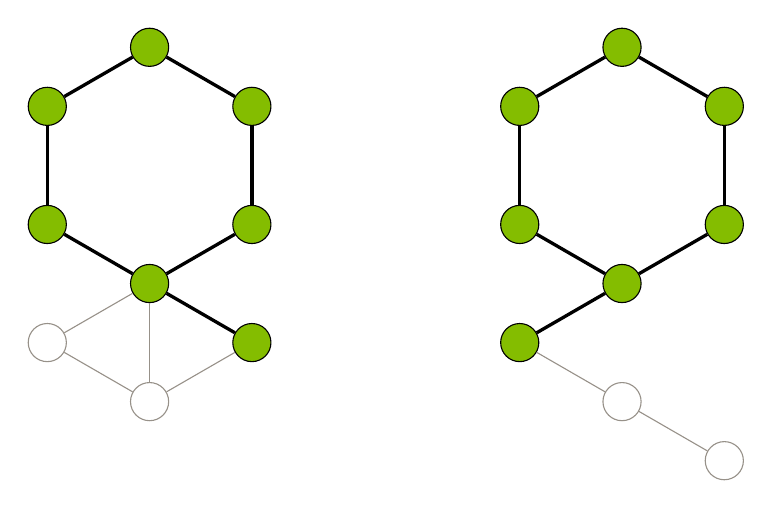
\begin{tikzpicture}
        \begin{scope}
            \node[draw, circle, fill=uofglawn, inner sep=2pt, font=\normalsize] (M1) at (90:1.5) {\phantom{0}};
            \node[draw, circle, fill=uofglawn, inner sep=2pt, font=\normalsize] (M2) at (150:1.5) {\phantom{0}};
            \node[draw, circle, fill=uofglawn, inner sep=2pt, font=\normalsize] (M3) at (30:1.5) {\phantom{0}};
            \node[draw, circle, fill=uofglawn, inner sep=2pt, font=\normalsize] (M4) at (210:1.5) {\phantom{0}};
            \node[draw, circle, fill=uofglawn, inner sep=2pt, font=\normalsize] (M5) at (330:1.5) {\phantom{0}};
            \node[draw, circle, fill=uofglawn, inner sep=2pt, font=\normalsize] (M6) at (270:1.5) {\phantom{0}};
            \node[draw, circle, draw=uofgsandstone!60, fill=white, inner sep=2pt, font=\normalsize] (M7) at ($(210:1.5) + (M6)$) {\phantom{0}};
            \node[draw, circle, fill=uofglawn, inner sep=2pt, font=\normalsize] (M8) at ($(330:1.5) + (M6)$) {\phantom{0}};
            \node[draw, circle, draw=uofgsandstone!60, fill=white, inner sep=2pt, font=\normalsize] (M9) at ($(270:1.5) + (M6)$) {\phantom{0}};

            \draw [very thick] (M1) -- (M2);
            \draw [very thick] (M2) -- (M4);
            \draw [very thick] (M3) -- (M5);
            \draw [very thick] (M4) -- (M6);
            \draw [very thick] (M5) -- (M6);
            \draw [very thick] (M3) -- (M1);
            \draw [color=uofgsandstone!60] (M6) -- (M7);
            \draw [very thick] (M6) -- (M8);
            \draw [color=uofgsandstone!60] (M6) -- (M9);
            \draw [color=uofgsandstone!60] (M7) -- (M9);
            \draw [color=uofgsandstone!60] (M8) -- (M9);
        \end{scope}

        \begin{scope}[xshift=6cm]
            \node[draw, circle, fill=uofglawn, inner sep=2pt, font=\normalsize] (M1) at (90:1.5) {\phantom{0}};
            \node[draw, circle, fill=uofglawn, inner sep=2pt, font=\normalsize] (M2) at (150:1.5) {\phantom{0}};
            \node[draw, circle, fill=uofglawn, inner sep=2pt, font=\normalsize] (M3) at (30:1.5) {\phantom{0}};
            \node[draw, circle, fill=uofglawn, inner sep=2pt, font=\normalsize] (M4) at (210:1.5) {\phantom{0}};
            \node[draw, circle, fill=uofglawn, inner sep=2pt, font=\normalsize] (M5) at (330:1.5) {\phantom{0}};
            \node[draw, circle, fill=uofglawn, inner sep=2pt, font=\normalsize] (M6) at (270:1.5) {\phantom{0}};
            \node[draw, circle, fill=uofglawn, inner sep=2pt, font=\normalsize] (M7) at ($(210:1.5) + (M6)$) {\phantom{0}};
            \node[draw, circle, draw=uofgsandstone!60, fill=white, inner sep=2pt, font=\normalsize] (M8) at ($(270:1.5) + (M6)$) {\phantom{0}};
            \node[draw, circle, draw=uofgsandstone!60, fill=white, inner sep=2pt, font=\normalsize] (M9) at ($(330:1.5) + (M8)$) {\phantom{0}};

            \draw [very thick] (M1) -- (M2);
            \draw [very thick] (M2) -- (M4);
            \draw [very thick] (M3) -- (M5);
            \draw [very thick] (M4) -- (M6);
            \draw [very thick] (M5) -- (M6);
            \draw [very thick] (M3) -- (M1);
            \draw [very thick] (M6) -- (M7);
            \draw [draw=uofgsandstone!60] (M7) -- (M8);
            \draw [draw=uofgsandstone!60] (M8) -- (M9);
        \end{scope}
\end{tikzpicture}}
\end{frame}

\begin{frame}{Who Cares?}
    \begin{itemize}
        \item Chemistry, biochemistry, and drug design (graphs are molecule fragments or proteins).
        \item Computer vision.
        \item Compilers (instruction generation, code rewriting).
        \item Plagiarism and malware detection.
        \item Livestock epidemiology (contact and trade graphs).
        \item Designing mechanical lock systems.
    \end{itemize}
\end{frame}

\begin{frame}{In Theory\ldots}
    \begin{itemize}
        \item Subgraph finding is hard.
        \item Subgraph counting is hard.
        \item Approximate subgraph finding is hard.
    \end{itemize}
\end{frame}

\begin{frame}{In Practice\ldots}
    \begin{itemize}
        \item We have good \emph{solvers} for subgraph problems.
        \item Some applications involve solving thousands of subgraph isomorphism queries per second.
        \item We can solve clique on larger graphs than we can solve all-pairs
            shortest path.\footnote{Terms and conditions apply.}
        \item<2-> Maximum common subgraph is still a nightmare\ldots
    \end{itemize}
\end{frame}

\section{In The Beginning\ldots}

\begin{frame}{Ancient History}
    \begin{itemize}
        \item Second DIMACS Implementation Challenge, 1992-93.
            \begin{itemize}
                \item Maximum clique.
                \item Graph colouring.
                \item Satisfiability.
            \end{itemize}
        \item ``Recent results in complexity theory have shown that, in a worst-case sense, the
            problems that are the subject of this Challenge are not only hard to solve optimally,
            they are hard to approximate.  Our goal in this Challenge is to provide an impetus for a
            coordinated attack on the question of how hard they are in practice.''
            \footnote{http://archive.dimacs.rutgers.edu/pub/challenge/call.txt}
    \end{itemize}
\end{frame}

\begin{frame}[fragile]{File Format}
\begin{lstlisting}
p edge 12 25             e 3 11
e 1 2                    e 4 6
e 1 5                    e 5 8
e 1 8                    e 6 7
e 1 10                   e 6 12
e 1 11                   e 7 9
e 1 12                   e 7 11
e 2 5                    e 7 12
e 2 8                    e 8 9
e 2 10                   e 9 10
e 3 4                    e 9 11
e 3 6                    e 9 12
e 3 10                   e 10 11
\end{lstlisting}
\end{frame}

\begin{frame}{Set of Instances}
    \begin{itemize}
        \item Random graphs with various sizes, densities, and models.
        \item Graphs with a large known clique hidden in a quasi-random graph.
        \item Fault diagnosis applications.
        \item Coding theory (Hamming, Johnson).
        \item Mathematical conjectures (Keller, Steiner triples).
    \end{itemize}
\end{frame}

\begin{frame}[fragile]{Experimental Protocol}
    \only<1>{
    ``BENCHMARKING: Whether you are studying exact or approximate algorithms, this code can serve as
    a simple benchmark for calibrating your machine's speed relative to those of the other
    participants.  If possible, please compile and run it on the supplied p=0.5 random graphs
    r100.5.b, r200.5.b, r300.5.b, r400.5.b, and r500.5.b and report your times.  For comparison
    purposes, the SGI Challenge "user" times (not counting input time) for one run on each graph
    were 0.08, 1.00, 7.87, 47.68, and 179.98 seconds, respectively.  The code can also be used as a
    common point of reference for papers implementing exact clique
    algorithms.''\footnote{http://archive.dimacs.rutgers.edu/pub/challenge/graph/solvers/README}
}\only<2>{
    \lstinputlisting[basicstyle=\scriptsize\ttfamily]{dfmax.txt}
}\only<3>{
    ``4. The CPU mark. In order to compensate for different processor speeds,
    Controller will standardize (i.e., scale) times according to the CPU marks
    provided by PassMark Single Thread Performance 3 . Currently, the top
    CPU mark is 3,255, while mid-range desktop processors have marks around
    2,000. So, we choose the mark 2,000 to define our standardized times.
    This means that if a run is performed in a processor Intel Core i9-9900T
    @ 2.10GHz that has mark 2,400, all local elapsed times will be multiplied
    by 1.2 to obtain the corresponding standardized times. This also means
    that a standardized time limit of 1,800 seconds will actually correspond
    to 1,500 seconds in that particular
    machine.''\footnote{http://dimacs.rutgers.edu/programs/challenge/vrp/cvrp/}
}
\end{frame}

\section{Maximum Clique Algorithms}

\begin{frame}{A Very Incomplete Guide to Maximum Clique Solvers}
    \begin{itemize}
        \item Since 1992, several papers per year.
        \item Many omissions, particularly of ideas that only showed up in one paper.
        \item Prosser, Algorithms 5(4) 2012 and my PhD thesis have more history.
    \end{itemize}
\end{frame}

\begin{frame}{Branch\ldots}
    \begin{itemize}
        \item Grow a maximum clique $A$, from the vertex set $P$:
        \item Pick a vertex $v$. Either $v$ is in a maximum clique:
            \begin{itemize}
                \item Let $P'$ be the set of vertices in $P$ that are adjacent to $v$.
                \item Recurse, finding a maximum clique in $A' = A \cup \{ v \}$ and $P'$.
            \end{itemize}
        \item Or it isn't. Throw out $v$ from $P$ and pick another $v$.
    \end{itemize}
\end{frame}

\begin{frame}{\ldots and Bound}
    \begin{itemize}
        \item Keep track of the largest clique found so far, the \emph{incumbent}, $\omega$.
        \item If $|C| + |P| \le \omega$, backtrack.
    \end{itemize}
\end{frame}

\begin{frame}{Degree Filtering}
    \begin{itemize}
        \item Every vertex in a clique of size $\omega$ has degree at least $\omega - 1$.
        \item Can calculate degree either in the original graph, or in $A \cup P$.
    \end{itemize}
\end{frame}

\begin{frame}{The Colour Bound}
    \only<1>{\begin{center}
    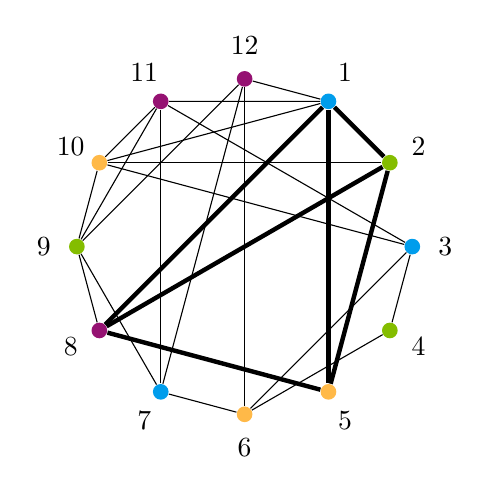
\begin{tikzpicture}
        \begin{scope}[scale=1.5]
        \newcount \myc
        \foreach \n in {1, 3, 7}{
            \myc=\n \advance\myc by -1 \multiply\myc by -360 \divide\myc by 12 \advance\myc by 60
            \node[anchor=center] (L\n) at (\the\myc:1.7) {\n};
            \node[anchor=center, circle, fill=uofgcobalt, inner sep=2pt] (N\n) at (\the\myc:1.42) {};
        }
        \foreach \n in {2, 4, 9}{
            \myc=\n \advance\myc by -1 \multiply\myc by -360 \divide\myc by 12 \advance\myc by 60
            \node[anchor=center] (l\n) at (\the\myc:1.7) {\n};
            \node[anchor=center, circle, fill=uofglawn, inner sep=2pt] (N\n) at (\the\myc:1.42) {};
        }
        \foreach \n in {5, 6, 10}{
            \myc=\n \advance\myc by -1 \multiply\myc by -360 \divide\myc by 12 \advance\myc by 60
            \node[anchor=center] (L\n) at (\the\myc:1.7) {\n};
            \node[anchor=center, circle, fill=uofgpumpkin, inner sep=2pt] (N\n) at (\the\myc:1.42) {};
        }
        \foreach \n in {8, 11, 12}{
            \myc=\n \advance\myc by -1 \multiply\myc by -360 \divide\myc by 12 \advance\myc by 60
            \node[anchor=center] (L\n) at (\the\myc:1.7) {\n};
            \node[anchor=center, circle, fill=uofgthistle, inner sep=2pt] (N\n) at (\the\myc:1.42) {};
        }
        \draw [ultra thick] (N1) -- (N2);
        \draw [ultra thick] (N1) -- (N5);
        \draw [ultra thick] (N1) -- (N8);
        \draw (N1) -- (N10);
        \draw (N1) -- (N11);
        \draw (N1) -- (N12);
        \draw [ultra thick] (N2) -- (N5);
        \draw [ultra thick] (N2) -- (N8);
        \draw (N2) -- (N10);
        \draw (N3) -- (N4);
        \draw (N3) -- (N6);
        \draw (N3) -- (N10);
        \draw (N3) -- (N11);
        \draw (N4) -- (N6);
        \draw [ultra thick] (N5) -- (N8);
        \draw (N6) -- (N7);
        \draw (N6) -- (N12);
        \draw (N7) -- (N9);
        \draw (N7) -- (N11);
        \draw (N7) -- (N12);
        \draw (N8) -- (N9);
        \draw (N9) -- (N10);
        \draw (N9) -- (N11);
        \draw (N9) -- (N12);
        \draw (N10) -- (N11);
    \end{scope}
    \end{tikzpicture}
    \end{center}}\only<2>{
    \begin{itemize}
        \item But how do we produce a colouring quickly?
            \begin{itemize}
                \item Greedily!
                \item But what order do we use for colouring the vertices?
            \end{itemize}
        \item More details: papers by Etsuji Tomita and co-authors.
        \item Interesting fact: the colour bound is \emph{strictly} better than degree.
    \end{itemize}}
\end{frame}

\begin{frame}{Colour Ordering}
    \only<1>{
        \centering
    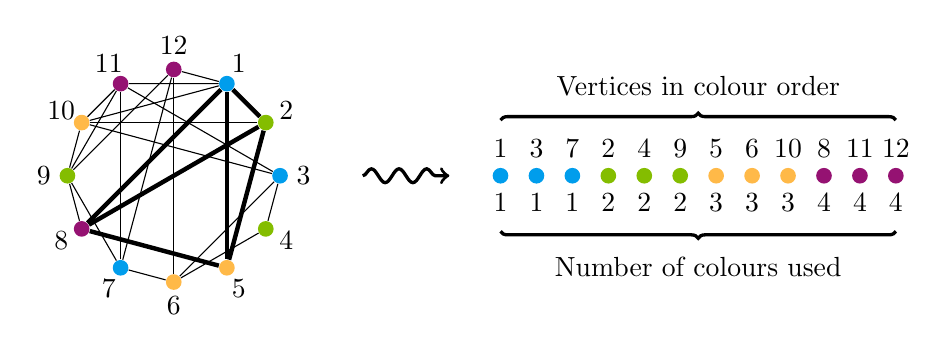
\begin{tikzpicture}
        \begin{scope}[scale=1.5]
        \newcount \myc
        \foreach \n in {1, 3, 7}{
            \myc=\n \advance\myc by -1 \multiply\myc by -360 \divide\myc by 12 \advance\myc by 60
            \node[anchor=center] (L\n) at (\the\myc:1.1) {\n};
            \node[anchor=center, circle, fill=uofgcobalt, inner sep=2pt] (N\n) at (\the\myc:0.9) {};
        }
        \foreach \n in {2, 4, 9}{
            \myc=\n \advance\myc by -1 \multiply\myc by -360 \divide\myc by 12 \advance\myc by 60
            \node[anchor=center] (l\n) at (\the\myc:1.1) {\n};
            \node[anchor=center, circle, fill=uofglawn, inner sep=2pt] (N\n) at (\the\myc:0.9) {};
        }
        \foreach \n in {5, 6, 10}{
            \myc=\n \advance\myc by -1 \multiply\myc by -360 \divide\myc by 12 \advance\myc by 60
            \node[anchor=center] (L\n) at (\the\myc:1.1) {\n};
            \node[anchor=center, circle, fill=uofgpumpkin, inner sep=2pt] (N\n) at (\the\myc:0.9) {};
        }
        \foreach \n in {8, 11, 12}{
            \myc=\n \advance\myc by -1 \multiply\myc by -360 \divide\myc by 12 \advance\myc by 60
            \node[anchor=center] (L\n) at (\the\myc:1.1) {\n};
            \node[anchor=center, circle, fill=uofgthistle, inner sep=2pt] (N\n) at (\the\myc:0.9) {};
        }
        \draw [ultra thick] (N1) -- (N2);
        \draw [ultra thick] (N1) -- (N5);
        \draw [ultra thick] (N1) -- (N8);
        \draw (N1) -- (N10);
        \draw (N1) -- (N11);
        \draw (N1) -- (N12);
        \draw [ultra thick] (N2) -- (N5);
        \draw [ultra thick] (N2) -- (N8);
        \draw (N2) -- (N10);
        \draw (N3) -- (N4);
        \draw (N3) -- (N6);
        \draw (N3) -- (N10);
        \draw (N3) -- (N11);
        \draw (N4) -- (N6);
        \draw [ultra thick] (N5) -- (N8);
        \draw (N6) -- (N7);
        \draw (N6) -- (N12);
        \draw (N7) -- (N9);
        \draw (N7) -- (N11);
        \draw (N7) -- (N12);
        \draw (N8) -- (N9);
        \draw (N9) -- (N10);
        \draw (N9) -- (N11);
        \draw (N9) -- (N12);
        \draw (N10) -- (N11);
    \end{scope}

\draw [processarrow] (2.4, 0) -> (3.5, 0);

\coordinate (Ms) at (3.8, 0.0);
\node[right = 0.35 of Ms,  anchor=center, circle, fill=uofgcobalt,  inner sep=2pt] (V1) {};
\node[right = 0.35 of V1,  anchor=center, circle, fill=uofgcobalt,  inner sep=2pt] (V2) {};
\node[right = 0.35 of V2,  anchor=center, circle, fill=uofgcobalt,  inner sep=2pt] (V3) {};
\node[right = 0.35 of V3,  anchor=center, circle, fill=uofglawn,    inner sep=2pt] (V4) {};
\node[right = 0.35 of V4,  anchor=center, circle, fill=uofglawn,    inner sep=2pt] (V5) {};
\node[right = 0.35 of V5,  anchor=center, circle, fill=uofglawn,    inner sep=2pt] (V6) {};
\node[right = 0.35 of V6,  anchor=center, circle, fill=uofgpumpkin, inner sep=2pt] (V7) {};
\node[right = 0.35 of V7,  anchor=center, circle, fill=uofgpumpkin, inner sep=2pt] (V8) {};
\node[right = 0.35 of V8,  anchor=center, circle, fill=uofgpumpkin, inner sep=2pt] (V9) {};
\node[right = 0.35 of V9,  anchor=center, circle, fill=uofgthistle, inner sep=2pt] (V10) {};
\node[right = 0.35 of V10, anchor=center, circle, fill=uofgthistle, inner sep=2pt] (V11) {};
\node[right = 0.35 of V11, anchor=center, circle, fill=uofgthistle, inner sep=2pt] (V12) {};
\node[above = 0.0 of V1] {1};
\node[above = 0.0 of V2] {3};
\node[above = 0.0 of V3] {7};
\node[above = 0.0 of V4] {2};
\node[above = 0.0 of V5] {4};
\node[above = 0.0 of V6] {9};
\node[above = 0.0 of V7] {5};
\node[above = 0.0 of V8] {6};
\node[above = 0.0 of V9] {10};
\node[above = 0.0 of V10] {8};
\node[above = 0.0 of V11] {11};
\node[above = 0.0 of V12] {12};
\node[below = 0.0 of V1] {1};
\node[below = 0.0 of V2] {1};
\node[below = 0.0 of V3] {1};
\node[below = 0.0 of V4] {2};
\node[below = 0.0 of V5] {2};
\node[below = 0.0 of V6] {2};
\node[below = 0.0 of V7] {3};
\node[below = 0.0 of V8] {3};
\node[below = 0.0 of V9] {3};
\node[below = 0.0 of V10] {4};
\node[below = 0.0 of V11] {4};
\node[below = 0.0 of V12] {4};

\draw[brace] ($(V1.north)+(0.0,0.6)$) -- ($(V12.north)+(0.0,0.6)$);
\node[anchor=south] at ($(V1)!0.5!(V12)$)[yshift=0.9cm] { Vertices in colour order };

\draw[brace] ($(V12.south)+(0.0,-0.6)$) -- ($(V1.south)+(0.0,-0.6)$);
\node[anchor=south] at ($(V1)!0.5!(V12)$)[yshift=-1.4cm] { Number of colours used };

    \end{tikzpicture}
    }\only<2->{
    \begin{itemize}
        \item Vertices in the rightmost colour class are ``generally expected [to have a] high
            probability of belonging to a maximum clique'' according to Tomita and Kameda, J. Global
            Optimization, 37(1) 2007.
        \item <3-> It's not true.
        \item <4-> Right to left is still better even if the algorithm is only proving optimality.
        \item <5-> Left to right finds larger solutions faster initially, but takes much longer
            overall.
    \end{itemize}}
\end{frame}

\begin{frame}{Greedy Colourings}
    \centering
    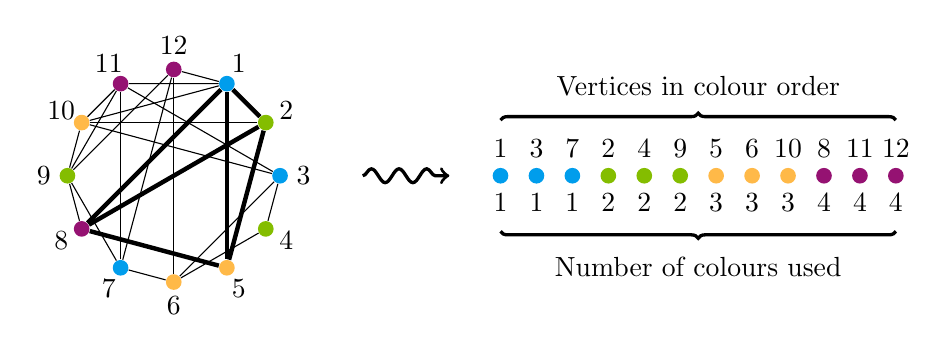
\begin{tikzpicture}
        \begin{scope}[scale=1.5]
        \newcount \myc
        \foreach \n in {1, 3, 7}{
            \myc=\n \advance\myc by -1 \multiply\myc by -360 \divide\myc by 12 \advance\myc by 60
            \node[anchor=center] (L\n) at (\the\myc:1.1) {\n};
            \node[anchor=center, circle, fill=uofgcobalt, inner sep=2pt] (N\n) at (\the\myc:0.9) {};
        }
        \foreach \n in {2, 4, 9}{
            \myc=\n \advance\myc by -1 \multiply\myc by -360 \divide\myc by 12 \advance\myc by 60
            \node[anchor=center] (l\n) at (\the\myc:1.1) {\n};
            \node[anchor=center, circle, fill=uofglawn, inner sep=2pt] (N\n) at (\the\myc:0.9) {};
        }
        \foreach \n in {5, 6, 10}{
            \myc=\n \advance\myc by -1 \multiply\myc by -360 \divide\myc by 12 \advance\myc by 60
            \node[anchor=center] (L\n) at (\the\myc:1.1) {\n};
            \node[anchor=center, circle, fill=uofgpumpkin, inner sep=2pt] (N\n) at (\the\myc:0.9) {};
        }
        \foreach \n in {8, 11, 12}{
            \myc=\n \advance\myc by -1 \multiply\myc by -360 \divide\myc by 12 \advance\myc by 60
            \node[anchor=center] (L\n) at (\the\myc:1.1) {\n};
            \node[anchor=center, circle, fill=uofgthistle, inner sep=2pt] (N\n) at (\the\myc:0.9) {};
        }
        \draw [ultra thick] (N1) -- (N2);
        \draw [ultra thick] (N1) -- (N5);
        \draw [ultra thick] (N1) -- (N8);
        \draw (N1) -- (N10);
        \draw (N1) -- (N11);
        \draw (N1) -- (N12);
        \draw [ultra thick] (N2) -- (N5);
        \draw [ultra thick] (N2) -- (N8);
        \draw (N2) -- (N10);
        \draw (N3) -- (N4);
        \draw (N3) -- (N6);
        \draw (N3) -- (N10);
        \draw (N3) -- (N11);
        \draw (N4) -- (N6);
        \draw [ultra thick] (N5) -- (N8);
        \draw (N6) -- (N7);
        \draw (N6) -- (N12);
        \draw (N7) -- (N9);
        \draw (N7) -- (N11);
        \draw (N7) -- (N12);
        \draw (N8) -- (N9);
        \draw (N9) -- (N10);
        \draw (N9) -- (N11);
        \draw (N9) -- (N12);
        \draw (N10) -- (N11);
    \end{scope}

\draw [processarrow] (2.4, 0) -> (3.5, 0);

\coordinate (Ms) at (3.8, 0.0);
\node[right = 0.35 of Ms,  anchor=center, circle, fill=uofgcobalt,  inner sep=2pt] (V1) {};
\node[right = 0.35 of V1,  anchor=center, circle, fill=uofgcobalt,  inner sep=2pt] (V2) {};
\node[right = 0.35 of V2,  anchor=center, circle, fill=uofgcobalt,  inner sep=2pt] (V3) {};
\node[right = 0.35 of V3,  anchor=center, circle, fill=uofglawn,    inner sep=2pt] (V4) {};
\node[right = 0.35 of V4,  anchor=center, circle, fill=uofglawn,    inner sep=2pt] (V5) {};
\node[right = 0.35 of V5,  anchor=center, circle, fill=uofglawn,    inner sep=2pt] (V6) {};
\node[right = 0.35 of V6,  anchor=center, circle, fill=uofgpumpkin, inner sep=2pt] (V7) {};
\node[right = 0.35 of V7,  anchor=center, circle, fill=uofgpumpkin, inner sep=2pt] (V8) {};
\node[right = 0.35 of V8,  anchor=center, circle, fill=uofgpumpkin, inner sep=2pt] (V9) {};
\node[right = 0.35 of V9,  anchor=center, circle, fill=uofgthistle, inner sep=2pt] (V10) {};
\node[right = 0.35 of V10, anchor=center, circle, fill=uofgthistle, inner sep=2pt] (V11) {};
\node[right = 0.35 of V11, anchor=center, circle, fill=uofgthistle, inner sep=2pt] (V12) {};
\node[above = 0.0 of V1] {1};
\node[above = 0.0 of V2] {3};
\node[above = 0.0 of V3] {7};
\node[above = 0.0 of V4] {2};
\node[above = 0.0 of V5] {4};
\node[above = 0.0 of V6] {9};
\node[above = 0.0 of V7] {5};
\node[above = 0.0 of V8] {6};
\node[above = 0.0 of V9] {10};
\node[above = 0.0 of V10] {8};
\node[above = 0.0 of V11] {11};
\node[above = 0.0 of V12] {12};
\node[below = 0.0 of V1] {1};
\node[below = 0.0 of V2] {1};
\node[below = 0.0 of V3] {1};
\node[below = 0.0 of V4] {2};
\node[below = 0.0 of V5] {2};
\node[below = 0.0 of V6] {2};
\node[below = 0.0 of V7] {3};
\node[below = 0.0 of V8] {3};
\node[below = 0.0 of V9] {3};
\node[below = 0.0 of V10] {4};
\node[below = 0.0 of V11] {4};
\node[below = 0.0 of V12] {4};

\draw[brace] ($(V1.north)+(0.0,0.6)$) -- ($(V12.north)+(0.0,0.6)$);
\node[anchor=south] at ($(V1)!0.5!(V12)$)[yshift=0.9cm] { Vertices in colour order };

\draw[brace] ($(V12.south)+(0.0,-0.6)$) -- ($(V1.south)+(0.0,-0.6)$);
\node[anchor=south] at ($(V1)!0.5!(V12)$)[yshift=-1.4cm] { Number of colours used };

    \end{tikzpicture}

    \begin{itemize}
        \item Branching on a colour class is like branching on a domain in CP, where the values are
            the vertices in the colour class plus a null value.
        \item Smallest domain first is a good heuristic.
        \item Greedy colourings tend to produce larger colour classes first.
        \item Right to left is smallest domain first.
    \end{itemize}
\end{frame}

\begin{frame}{We Can Measure This!}
    \centering\includegraphics<1>{graph-sortedness-shuffle.pdf}%
    \centering\includegraphics<2>{graph-sortedness-sorted.pdf}%
    \centering\includegraphics<3>{graph-sortedness-default.pdf}
\end{frame}

\begin{frame}{Increasing Sortedness Decreases Search Space Size}
    \centering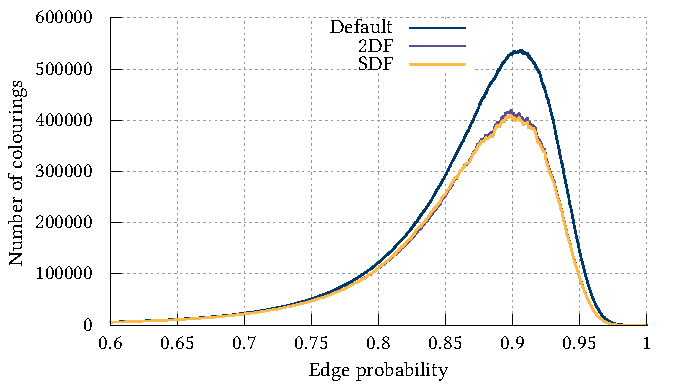
\includegraphics{graph-reorder-cumulative-nodes.pdf}
\end{frame}

\begin{frame}{However\ldots}
    \begin{itemize}
        \item Small impact on runtime.
        \item Hard to sell ``understanding why this algorithm works'' compared to ``this new
            algorithm is better''.
        \item John N. Hooker: ``Testing heuristics: We have it all wrong''. J. Heuristics 1(1) 1995.
    \end{itemize}
\end{frame}

\section{Maximum Clique Benchmark Instances}

\begin{frame}{Random Benchmark Instances}
    \begin{center}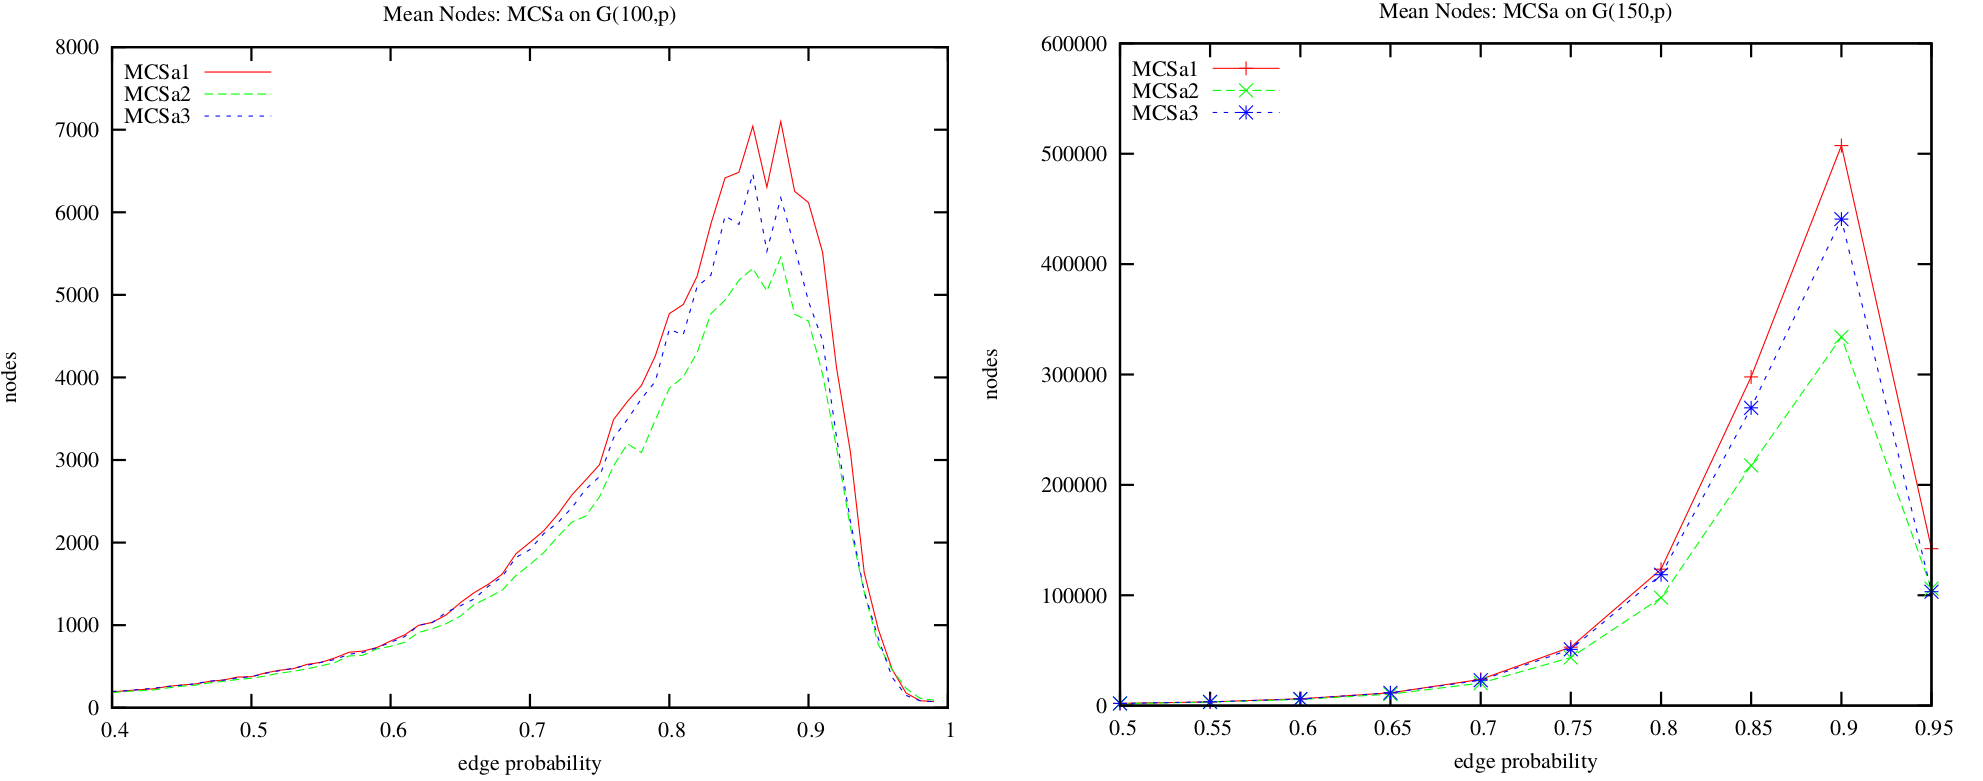
\includegraphics[keepaspectratio=true,scale=0.65]{prosser.png}\end{center}

    Prosser, Algorithms 5(4) 2012. Both plots have 100 samples per density step. The
    left-hand plot seems to go up in density steps of 0.01, and the right-hand plot, 0.05.
\end{frame}

\begin{frame}{Let's Measure This Properly}
    \includegraphics<1>{graph-optimisation.pdf}%
    \includegraphics<2>{graph-optimisation-1.pdf}%
    \includegraphics<3>{graph-optimisation-2.pdf}
\end{frame}

\begin{frame}{Phase Transitions}
    \centering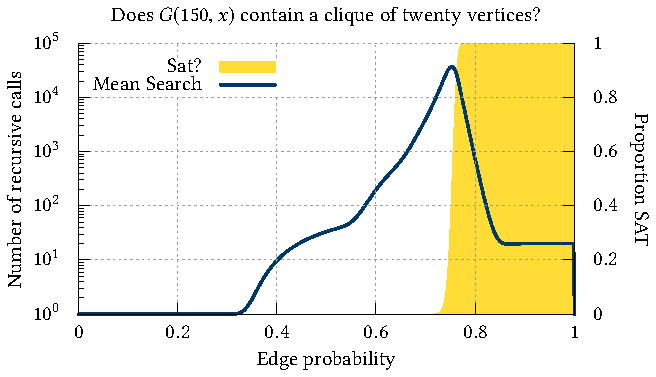
\includegraphics{graph-phase-transition.pdf}
\end{frame}

\begin{frame}{Intuition}
    \begin{itemize}
        \item Low density means no occurrences, and we can quickly show we run out of edges after
            doing a bit of branching.
        \item \only<1>{High density means lots of occurrences, so wherever we look, it's easy to find one of
            them.}\only<2>{\textcolor{uofgpillarbox}{High density means lots of occurrences, so wherever we look, it's
            easy to find one of them.}}
        \item If we expect there to be just one solution, it's really hard to find it if it
            exists, and really hard to rule it out if it doesn't exist.
    \end{itemize}
\end{frame}


\begin{frame}{Optimisation versus Decision}
    \includegraphics<1>{graph-waves-0.pdf}%
    \includegraphics<2>{graph-waves.pdf}%
    \includegraphics<3>{graph-waves-1.pdf}%
    \includegraphics<4>{graph-waves-2.pdf}%
    \includegraphics<5>{graph-waves-3.pdf}%
\end{frame}

\begin{frame}{Finding versus Proving Optimality}
    \includegraphics<1>{graph-waves-0.pdf}%
    \includegraphics<2>{graph-find-prove.pdf}%
    \includegraphics<3>{graph-find-prove-1.pdf}%
\end{frame}

\begin{frame}{Difficulty by Solution Size}
    \includegraphics<1>{graph-by-omega.pdf}%
    \includegraphics<2>{graph-by-omega-1.pdf}%
    \includegraphics<3>{graph-by-omega-2.pdf}%
    \includegraphics<4>{graph-by-omega-3.pdf}%
    \includegraphics<5>{graph-by-omega-4.pdf}%
\end{frame}

\begin{frame}{Difficulty by Optimal Solution Frequency}
    \includegraphics<1>{graph-omega-20-0.pdf}%
    \includegraphics<2>{graph-omega-20-1.pdf}%
    \includegraphics<3>{graph-omega-20-2.pdf}%
    \includegraphics<4>{graph-omega-20-3.pdf}%
    \includegraphics<5>{graph-omega-60-3.pdf}%
\end{frame}

\begin{frame}{Search Order}
    \includegraphics<1>{graph-anti-0.pdf}%
    \includegraphics<2>{graph-anti-1.pdf}%
    \includegraphics<3>{graph-anti-2.pdf}%
\end{frame}

\begin{frame}{First Solution Quality}
    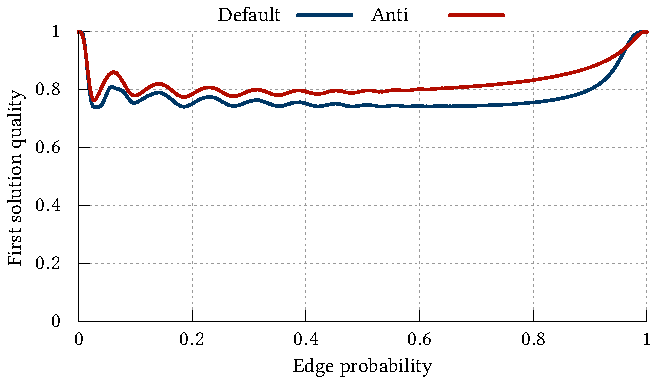
\includegraphics{graph-fsq.pdf}
\end{frame}

\begin{frame}{Solution Quality over Time}
    \includegraphics<1>{graph-sqot.pdf}%
    \includegraphics<2>{graph-sqot-rco.pdf}%
\end{frame}

\begin{frame}{Priming}
    \begin{itemize}
        \item Run local search before starting the main algorithm, to get a good initial incumbent.
        \item ``We run the ILS heuristic with 100000 scans for all the considered instances except
            gen400\_p0.9\_55 and p\_hat1000-3 for which we use 60 millions scans because these two
            instances are computationally difficult.'', Maslov et al, J. Global Optimization, 59(1)
            2014.
        \item More details: papers by Etsuji Tomita and Pablo San Segundo.
    \end{itemize}
\end{frame}

\begin{frame}{The DIMACS Instances}
    \begin{itemize}
        \item Heavy bias towards ``large hidden solution'' instances and random instances.
            \begin{itemize}
                \item If you can find the large hidden solution, proving optimality is easy.
            \end{itemize}
        \item The application instances are extremely easy.
        \item Still a few open instances, and a few more that can only be solved with years of CPU
            time.
        \item Sufficiently few hard instances that, e.g.\ random permutations can easily change which
            algorithm is ``state of the art''.
            \begin{itemize}
                \item Particularly on the ``large hidden clique'' instances.
            \end{itemize}
        \item Still widely used.
    \end{itemize}
\end{frame}

\begin{frame}{Large Sparse Graphs}
    \begin{itemize}
        \item Biggest DIMACS graph: 4,000 vertices, density 0.5.
            \begin{itemize}
                \item This will fit in an adjacency matrix.
            \end{itemize}
        \item Often claimed that large sparse graphs are ``more realistic''.
            \begin{itemize}
                \item Not immediately clear why anyone would want to find a clique in a road
                    network\ldots
            \end{itemize}
    \end{itemize}
\end{frame}

\section{Other Clique Problems}

\begin{frame}{Enumeration}
    \begin{itemize}
        \item Output all maximal cliques.
        \item Several published tables of results are wrong\ldots
    \end{itemize}
\end{frame}

\begin{frame}{Weighted Clique}
    \begin{itemize}
        \item Vertices have weights.
            \begin{itemize}
                \item Weighted colour bounds?
            \end{itemize}
        \item Lack of good benchmark instances, so authors reuse DIMACS graphs and assign weight $v
            \operatorname{mod} 200 + 1$ to vertex $v$.
        \item Why this is bad, and better instances: McCreesh et al, CP 2017.
    \end{itemize}
\end{frame}

\section{Subgraph Isomorphism}

\begin{frame}{Crimes Too Gory For This Talk}
    \begin{itemize}
        \item To generate benchmark instances: create a large sparse random graph, pick a random
            connected subgraph.
            \begin{itemize}
                \item All satisfiable.
                \item Trivial for a CP solver.
                \item Hard for non-CP algorithms that have a better marketing department.
            \end{itemize}
        \item Build ``filter + verify'' systems to detect obviously infeasible instances, because
            the algorithms are so bad.
        \item Include duplicates of all of the queries in datasets, and then publish papers saying
            that caching query results can be really beneficial.
        \item Realise you're still losing to CP, and start publishing papers on ``whose solver can
            find 1,000 solutions fastest'' where you measure who has the most optimised print
            statements.
        \item Cite my JAIR 2015 paper that explains why all of the benchmark instances are bad and
            why this matters, claim it says the opposite of what it actually does, and carry on
            doing the same thing anyway.
    \end{itemize}
\end{frame}

\section{Conclusion}

\begin{frame}{A Summary of Crimes Witnessed}
    \begin{itemize}
        \item Buggy solvers
        \item Excessive parameter tuning
        \item Hard-coding parameters based upon instance filenames
        \item Badly-generated random benchmark sets
        \item Badly-generated non-random benchmark sets
        \item Reuse of good benchmark instances from other problems in a way that makes them bad
        \item Moving goalposts until you're benchmarking whose print statement is fastest
        \item Multiplying other people's runtimes by mysterious scaling factors rather than re-running experiments
        \item Entire systems built on top of not understanding the theory correctly
    \end{itemize}
\end{frame}

\begin{frame}{Concluding Troublemaking}
    \begin{itemize}
        \item The algorithm engineering community sucks at benchmarking.
        \item The algorithm engineering community sucks at measurement.
        \item The algorithm engineering community sucks at understanding.
        \item The graph databases community is even worse.
        \item At least some of the automated reasoning community are somewhat better some of the
            time.
    \end{itemize}
\end{frame}

{
    \usebackgroundtemplate{
        \tikz[overlay, remember picture]
        \node[at=(current page.south), anchor=south, inner
        sep=0pt]{\includegraphics[keepaspectratio=true, width=\paperwidth]{background2.jpg}};
    }

    \begin{frame}[plain,noframenumbering]
        \begin{tikzpicture}[remember picture, overlay]
            \node at (current page.north west) {
                \begin{tikzpicture}[remember picture, overlay]
                    \fill [fill=uofguniversityblue, anchor=north west] (0, 0) rectangle (\paperwidth, -2.6cm);
                \end{tikzpicture}
            };

            \node (logo) [anchor=north east, shift={(-0.6cm,-0.6cm)}] at (current page.north east) {
                
\includegraphics[keepaspectratio=true,scale=0.7]{UoG_keyline.pdf}
            };

            \node [anchor=north west, shift={(0.6cm,-0.8cm)}] at (current page.north west) {
                \textcolor{white}{\url{https://ciaranm.github.io/}}
            };

            \node [anchor=north west, shift={(0.6cm,-1.4cm)}] at (current page.north west) {
                    \textcolor{white}{\href{mailto:ciaran.mccreesh@glasgow.ac.uk}{\nolinkurl{ciaran.mccreesh@glasgow.ac.uk}}}
            };
        \end{tikzpicture}
    \end{frame}
}

{
    \usebackgroundtemplate{
        \tikz[overlay, remember picture]
        \node[at=(current page.south), anchor=south, yshift=-1cm, inner sep=0pt]{\includegraphics[keepaspectratio=true, width=\paperwidth]{../../images/background2.jpg}};
    }

    \begin{frame}[plain,noframenumbering]
        \begin{tikzpicture}[remember picture, overlay]
            \node at (current page.north west) {
                \begin{tikzpicture}[remember picture, overlay]
                    \fill [fill=uofguniversityblue, anchor=north west] (0, 0) rectangle (\paperwidth, -2.8cm);
                \end{tikzpicture}
            };

            \node (logo) [anchor=north east, shift={(-0.8cm,-0.2cm)}] at (current page.north east) {
                
\includegraphics[keepaspectratio=true,scale=0.5]{../../images/UoG_keyline.pdf}
            };

            \node (logo2) [anchor=north, below=0.2cm of logo.south] {
                
\includegraphics[keepaspectratio=true,scale=0.1]{../../images/RAEngWhite.pdf}
            };

            \coordinate (logos) at ($(logo.south)!0.5!(logo2.north)$);

            \node [anchor=west, xshift=0.8cm] at (current page.west |- logos) {
                \begin{minipage}{0.60\paperwidth}\raggedright
                    \textcolor{white}{\url{https://ciaranm.github.io/}} \\[0.3cm]
                    \textcolor{white}{\href{mailto:ciaran.mccreesh@glasgow.ac.uk}{\nolinkurl{ciaran.mccreesh@glasgow.ac.uk}}}
                \end{minipage}
            };
        \end{tikzpicture}
    \end{frame}
}

\end{document}

